\documentclass[a4paper, 12pt]{scrreprt}
%Schriftart
\usepackage{fontspec}
%\usepackage[utf8]{inputenc}
%\usepackage[T1]{fontenc}
\usepackage[ngerman]{babel}

%Festlegen des Seitenlayouts
\usepackage[onehalfspacing]{setspace} %Zeilenabstand
%alternativ \linespread{1.5}
%BCOR ist der Binderand, DIV definiert den Satzspiegel (siehe KOMA-script Dokumentation S. 30)
\KOMAoptions{BCOR=0.5cm, DIV=11, parskip=half}
%Absätze werden über parskip geregelt. Die Werte sind parskip=true/false/half

%Abstand vor Kapitelbeginn
\RedeclareSectionCommand[
  beforeskip=0pt,
  afterindent=false
]{chapter}

%Schriftart der Überschriften serif in bold
\addtokomafont{disposition}{\rmfamily}
%Schriftart der Überschriften in serif ohne bold
%\setkomafont{disposition}{\normalfont}

%Für das Einfügen eines Glossars: siehe https://en.wikibooks.org/wiki/LaTeX/Glossary

%stützt die Schnittstelle von float und listings zu tocbasic (genutzt von KOMA-script)
\usepackage{scrhack}

%Zum Auskommentieren von größeren Blöcken
\usepackage{comment}
%Als Platzhalter
\usepackage{lipsum}
%Einfachere Verwendung von Anführungszeichen
\newcommand{\qt}[1]{\glqq#1\grqq{}}
%Angabe von Bildquellen
\newcommand{\quelle}[1]{\\\vspace{.1cm}{Quelle: #1}}

\setcounter{tocdepth}{2}  % show subsections


%Bilder
\usepackage{graphicx}
\usepackage{float}
\graphicspath{{./abbildungen/}}
\usepackage{tabularx}


%Einfügen von Unformatiertem typewriter Text
\usepackage{verbatim}
%über mehrere Zeilen mit \begin{Verbatim}[breaklines=true]\end{Verbatim}
\usepackage{fancyvrb}
\usepackage{makecell}

%Alles was das Formelherz begehrt
\usepackage{amstext} 
\usepackage{amsmath}
\usepackage{amssymb}
\usepackage{booktabs}

%Für die Literaturverzeichnisse
\usepackage{csquotes}
\usepackage[
backend=biber,
style=authoryear,
sorting=nyt,
autocite=footnote,
maxcitenames=2,
dashed=false
]{biblatex}

% Format all names as Family, Given
\DeclareNameAlias{sortname}{family-given}

% Separate authors with semicolons instead of commas
\DeclareDelimFormat{multinamedelim}{\addsemicolon\space}
\DeclareDelimFormat{finalnamedelim}{\addspace\bibstring{and}\space} % uses "und" before the last name

\DefineBibliographyStrings{german}{
	andothers = {et\ al.},
	urlseen   = {Abrufdatum: },
}
\addbibresource{lit.bib}

\setlength{\bibhang}{0pt}
\renewbibmacro*{begentry}{%
	\ifkeyword{bild}{}{\ensuremath{\bullet}\space}%
}

\defbibenvironment{bildliste}
{\list{}
	{\setlength{\leftmargin}{3.5cm}%
		\setlength{\itemindent}{-3.5cm}%
		\setlength{\itemsep}{\bibitemsep}%
		\setlength{\parsep}{\bibparsep}}}
{\endlist}
{\item[]\textbf{\printfield{label}:}\addspace}
%Literaturverzeichnis exakt nach ISO 690-3
%Eine Alternative Erstellung von Literaturverzeichnissen über natbib (letzte Version von 2010)
%WICHTIG: bei einem Wechsel müssen alle Temporären Dateien von LaTex gelöscht werden!
%\usepackage{natbib}
%\usepackage{multibib} %Unterteilung in Internet- und Printmedien
%\newcites{online}{Internetquellenverzeichnis} 
%Statt \cite{} muss für Internetquellen nun \citeonline{} verwendet werden!

\DeclareSortingTemplate{bylabel}{
	\sort{\field{label}}
	\sort{\field{sortname}\field{author}\field{editor}\field{translator}}
	\sort{\field{year}}
	\sort{\field{title}}
}

%Anklickbare Links und \url{}
\usepackage[hidelinks]{hyperref}

\usepackage{xurl}


%Zeilenumbrüche in URLs, standard url Paket wird von hyperref geladen, Befehl \url{} bleibt gleich
\usepackage{microtype}[final]

\usepackage{chngcntr}
\counterwithout{footnote}{chapter}
%Einbinden von Quelltext in Python (https://tex.stackexchange.com/questions/83882/how-to-highlight-python-syntax-in-latex-listings-lstinputlistings-command)
% Default fixed font does not support bold face
\DeclareFixedFont{\ttb}{T1}{txtt}{bx}{n}{12} % for bold
\DeclareFixedFont{\ttm}{T1}{txtt}{m}{n}{12}  % for normal

% Custom colors
\usepackage{color}
\definecolor{deepblue}{rgb}{0,0,0.5}
\definecolor{deepred}{rgb}{0.6,0,0}
\definecolor{deepgreen}{rgb}{0,0.5,0}

\usepackage{listings}

% Python style for highlighting
\newcommand\pythonstyle{\lstset{
language=Python,
basicstyle=\ttm,
otherkeywords={self},             % Add keywords here
keywordstyle=\ttb\color{deepblue},
emph={MyClass,__init__},          % Custom highlighting
emphstyle=\ttb\color{deepred},    % Custom highlighting style
stringstyle=\color{deepgreen},
frame=tb,                         % Any extra options here
showstringspaces=false            % 
}}


% Python environment
\lstnewenvironment{python}[1][]
{
\pythonstyle
\lstset{#1}
}
{}

% Python for external files
\newcommand\pythonexternal[2][]{{
\pythonstyle
\lstinputlisting[#1]{#2}}}

% Python for inline
\newcommand\pythoninline[1]{{\pythonstyle\lstinline!#1!}}



\begin{document}
\hypersetup{pageanchor=false}
\begin{titlepage}
\thispagestyle{empty}
\vspace{-1cm}
\begin{center}
    \vspace{-2cm}
    
\includegraphics[width=0.3\textwidth]{czg.pdf}
\end{center}

\begin{center}
 \begin{spacing}{1.0}
 
 \Huge{\textbf{Autoantikörper gegen Caspr2 }}\\
 {\Large eine immunhistologische Analyse ihrer Auswirkungen im zentralen Nervensystem}\\
 \end{spacing}
 \vspace{1cm}
 \begin{spacing}{1.0}
 {\normalsize Seminarfacharbeit in den Spezialklassen mit mathematisch-naturwissenschaftlich-technischer Richtung der gymnasialen Oberstufe}
\end{spacing}
\end{center}

\vspace{0.4cm} %diesen Wert ändern, wenn der Titel sehr lang ist
\begin{spacing}{1.1}
\large{
\begin{flushleft}
\begin{tabular}{ll}
Autor/ -innen: & Johanna Hoppe\\ 
 & Helene Becker\\ 
 & Kushagr Sinha\\
\noalign{\vskip 5mm}    
Schule: & Carl-Zeiss-Gymnasium Jena\\
\noalign{\vskip 5mm}
Abgabetermin: & 30. September 2026\\
\noalign{\vskip 5mm}    
Fachbetreuerinnen: & Frau Dr. Josefine Sell\\
 & Frau Dr. Anja Strauß\\
\noalign{\vskip 5mm}    
 Fachlehrerin: & Frau Sybille Weiß\\
\noalign{\vskip 5mm}
Betreuerin: & Frau Dr. Annett Fiedler\\
\noalign{\vskip 5mm}  
\end{tabular}
\end{flushleft}
}
\end{spacing}

\end{titlepage}


\pagenumbering{roman}
\tableofcontents


\chapter{Motivation und Zielsetzung}
\pagenumbering{arabic}
\textbf{Johanna Hoppe}


Entzündungen des Gehirns (Enzephalitis) werden meist durch Bakterien
oder Viren ausgelöst. Seltener ist eine Fehlreaktion des Immunsystems
der Grund.

Die Autoimmune Enzephalitis ist eine neurologische Erkrankung, die durch
Autoantikörper gegen neuronale Oberflächenproteine ausgelöst wird. Diese
fehlgeleitete Immunreaktion des Körpers führt zu einer beeinträchtigten
Signalweiterleitung am Axon und einer gestörten synaptischen
Übertragung. Dies äußert sich durch Symptome wie Gedächtnisstörungen, psychiatrischen Auffälligkeiten, oder Wesensverändernung. Betroffene leiden häufig
an verzögerter Muskelentspannung nach willkürlicher Muskelanspannung,
epileptischen Anfällen sowie Schlafstörungen und kognitiven
Defiziten.\footcite{VanSonderenNatRev2016}

Der Fokus der vorliegenden Arbeit liegt auf der autoimmunen
Caspr2-Enzephalitis, bei der Autoantikörper gegen das neuronale Protein
Contactin-associated protein 2 (Caspr2) gebildet werden. Caspr2 bildet mit Kaliumionenkanälen und
weiteren Proteinen im Nervensystem Komplexe, welche unter anderem für
die Lokalisation der Kaliumionenkanäle relevant sind. Bekannt ist
bereits, dass Caspr2 für die funktionierende Signalweiterleitung durch
das Axon von Bedeutung ist. Studien konnten Caspr2 2008 ebenfalls an Synapsen, den Verbindungsstellen zwischen zwei Nervenzellen, nachweisen. Der Fokus dieser Arbeit liegt daher auf der
Untersuchung von Caspr2 und der Wirkung von Autoantikörpern gegen
dieses Protein an den Synapsen des zentralen Nervensystems. In
Zusammenarbeit mit Dr.~Josefine Sell vom Universitätsklinikum Jena
werden zwei Teiluntersuchungen
durchgeführt.

Zum einen soll herausgefunden werden, ob Caspr2 eher an erregenden (exzitatorischen) oder
hemmenden (inhibitorischen) Synapsen lokalisiert ist. Dazu werden an
Hippocampuszellkulturen von Mäusen Doppelfärbungen kommerzieller
Caspr2-Antikörper mit je einem der synaptischen Marker VGlut1 (für
exzitatorische Synapsen) und VGat (für inhibitorische Synapsen)
durchgeführt. Diese werden mithilfe hochauflösender
Fluoreszenzmikroskopie analysiert und ausgewertet.

Im zweiten Teil wird untersucht, ob Antikörper gegen Caspr2 die
Interaktion zwischen Caspr2 und seinem Bindungspartner Contactin-2
stören. Dafür werden lebende neuronale Zellkulturen mit aus Patienten gewonnenen 
Caspr2-Antikörpern behandelt. Anschließend erfolgt eine Doppelfärbung
von Caspr2 und Contactin-2, um mögliche Veränderungen in der
Kolokalisation der beiden Proteine festzustellen.

Ziel dieser Seminarfacharbeit ist es, durch die Untersuchungen dazu
beizutragen, ein besseres Verständnis für die Caspr2-assoziierte
Enzephalitis zu entwickeln. Denn nur wenn die zugrundeliegenden Vorgänge
im Gehirn genau verstanden werden, kann die Diagnostik und Behandlung
der Krankheit weiter optimiert werden.
\chapter{Grundlagen}

\section{Neurobiologische Grundlagen}
\textbf{Johanna Hoppe}
%\subsection{Aufbau und Funktion des Nervensystems}
%Das Nervensystem des Menschen lässt sich funktionell und topographisch
%unterteilen. Man unterscheidet das zentrale Nervensystem (ZNS), welches
%Informationen verarbeitet, und das periphere Nervensystem (PNS), welches
%Informationen zum zentralen Nervensystem sowie zu Muskel- oder
%Drüsenzellen leitet.\footcite{Westphalen2004}
%
%Das zentrale Nervensystem besteht aus dem Rückenmark und dem
%Gehirn. Das Rückenmark liegt im Inneren der Wirbelsäule und
%besteht aus Axonbündeln, wodurch es vor allem eine Leitungsbahn zwischen
%dem Gehirn und dem restlichen Körper darstellt. Es steuert außerdem
%koordinierte Bewegungen wie Laufen und löst einfache Reflexe aus, wie
%zum Beispiel den Lidschluss- und den
%Kniesehnenreflex.\footcite{Freedman2025Rueckenmark}
%
%Am oberen Ende des Rückenmarks schließt sich im Bereich der Medulla
%oblongata der Hirnstamm und damit das Gehirn an. Der Bau des
%Gehirns lässt sich in Vorderhirn und Hirnstamm einteilen. Das
%Vorderhirn besteht aus dem Zwischenhirn, also dem Thalamus und dem
%Hypothalamus, und dem Großhirn. Der Hirnstamm wird in Mittelhirn und
%Rautenhirn, welches unter anderem das Kleinhirn einschließt, unterteilt.
%Diese Zusammenhänge sind in Abbildung \ref{fig:anaNBG}
%dargestellt.\footcite[S.~1105]{Markl1997}
%\clearpage
%% ── Abbildung 1 ausgelassen ──────────────────────────────────
%% Abbildung 1: Aufbau des Gehirns
%% Quelle: \cite[S.~1105]{Markl1997}
%% ─────────────────────────────────────────────────────────────
%\begin{figure}[h] % [h] versucht, das Bild hier zu platzieren (hier), [t] für oben, [b] für unten
%	\centering % Zentriert das Bild horizontal
%	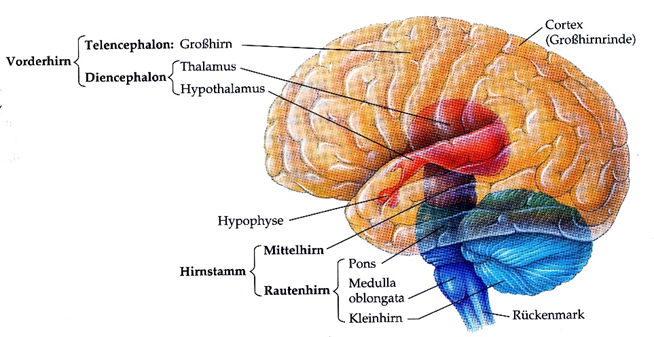
\includegraphics[width=0.8\textwidth]{abbildungen/anatomieNBG.png} % Lädt das Bild, skaliert es auf 80% der Textbreite
%	\caption{ Aufbau des Gehirns \parencite{MarklBild1997a}} % Die Bildunterschrift
%	\label{fig:anaNBG} % Ein Label für Querverweise (z.B. "siehe Abbildung \ref{fig:beispielbild}")
%\end{figure}
%
%Das Kleinhirn liegt hinter bzw.\ unter dem Großhirn. Seine
%Hauptfunktion liegt in der Koordination von Bewegungen. So enthält es
%beispielsweise Informationen zur Stellung der Gelenke oder Länge der
%Muskeln und kann, nach Input des Großhirns über motorische Ausgänge, die
%automatische Koordination von Körperbewegungen und die Balance steuern.
%Durch das Kleinhirn wird also ein fließender und abgestimmter
%Bewegungsablauf ermöglicht, der zum Beispiel bei der
%Auge-Hand-Koordination von Bedeutung
%ist.\footcite[S.~1106]{Markl1997}
%
%Einige Teile des Zwischenhirns und des Großhirns bilden das
%limbische System, das unter anderem den Hippocampus umfasst.
%Der Hippocampus ist eine paarig angelegte Struktur. Er befindet
%sich am Innenrand des Temporallappens und an den Seitenventrikeln. Der
%Hippocampus spielt eine entscheidende Rolle bei der Gedächtnisbildung.
%Insbesondere ist er an der Konsolidierung von Gedächtnisinhalten
%beteiligt, also an der Überführung neuer Informationen aus dem
%Kurzzeitgedächtnis in das Langzeitgedächtnis. Darüber hinaus ist er von
%Bedeutung für das räumliche Gedächtnis sowie für Lernprozesse. Durch
%seine Einbindung in das limbische System ist er ebenfalls an Funktionen
%wie Emotionen und Motivation
%beteiligt.\footcite{Hoegemann2006}
%
%Das periphere Nervensystem bildet den zweiten großen Bestandteil
%des menschlichen Nervensystems. Topografisch gliedert es sich in die
%Hirnnerven und die Spinalnerven. Der Mensch besitzt zwölf
%Hirnnervenpaare, welche direkt aus dem Gehirn austreten und vor allem
%den Kopf- und Halsbereich versorgen, sowie 31 Spinalnervenpaare, die aus
%dem Rückenmark hervorgehen und in den Rumpf, die Extremitäten und die
%inneren Organe führen. Diese peripheren Nerven bestehen jeweils
%aus Bündeln vieler Neuronen. Das periphere Nervensystem setzt sich aus
%zwei funktionellen Untereinheiten zusammen. Die sensorische Untereinheit
%leitet Informationen von Sinneszellen oder inneren Organen zum zentralen
%Nervensystem. Dies findet beispielsweise bei dem Registrieren von Wärme
%oder Kälte statt. Die motorische Untereinheit hingegen überträgt Signale
%aus dem zentralen Nervensystem an die Effektoren, also zu Muskel- oder
%Drüsenzellen. Der motorische Anteil des peripheren Nervensystems kann
%weiter in das somatische und das autonome Nervensystem gegliedert
%werden, wobei das somatische Nervensystem bewusste Bewegungen steuert,
%während das autonome Nervensystem durch das Zusammenwirken von
%Sympathicus und Parasympathicus unwillkürliche Prozesse wie
%beispielsweise den Herzschlag
%reguliert.\footcite[S.~1100--1102]{Markl1997}


\subsection{Signalweiterleitung am Axon und synaptische Signalübertragung}

Um die Rolle bestimmter Proteine für die Signalweiterleitung in einer
Nervenzelle zu verstehen, sollen der Aufbau einer Nervenzelle sowie der
Prozess der Signalweiterleitung genauer betrachtet werden.

Die grundlegende Funktionseinheit des Nervensystems ist die
Nervenzelle, auch Neuron genannt.

\begin{figure}[h] % [h] versucht, das Bild hier zu platzieren (hier), [t] für oben, [b] für unten
	\centering % Zentriert das Bild horizontal
	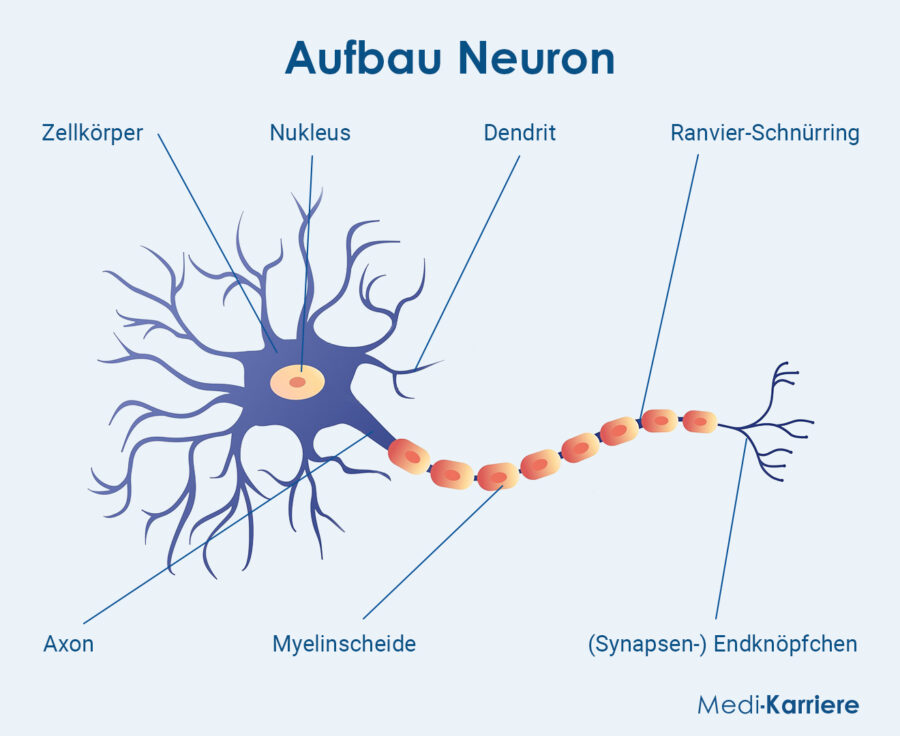
\includegraphics[width=0.7\textwidth]{NEU1bild.jpg} % Lädt das Bild, skaliert es auf 80% der Textbreite
	\caption{ Aufbau einer Nervenzelle \parencite{MediKarriere2024}} % Die Bildunterschrift
	\label{fig:NEU1} % Ein Label für Querverweise (z.B. "siehe Abbildung \ref{fig:beispielbild}")
\end{figure}

Ein Neuron besteht aus einem Zellkörper (Soma), welcher das Zellplasma,
den Zellkern sowie weitere typische Zellorganellen enthält. (Zwischen dem Zellinneren und dem äußeren Milieu gibt es unterschiedliche Ionenzusammensetzungen, die zum Teil von der Zelle aktiv aufrecht erhalten werden. (Durch die unterschiedlichen positiven und negativen Ladungen und den chemischen Gradienten entsteht an der Membran ein Potential, das Membranpotential). Das Zellinnere ist dabei im Vergleich zum Zelläußeren negativ geladen, das Zelläußere positiv.) Vom Zellkörper gehen Dendriten, verzweigte Fortsätze des Neurons, aus, die der
Aufnahme eingehender Signale anderer Neuronen dienen. Sie leiten Signale
elektrisch zum Zellkörper weiter. Am Übergang zum Axon, dem Axonhügel,
werden die eingehenden Signale summiert.  Über das Axon werden elektrische Spannungsänderungen bis zu den synaptischen Endigungen weitergeleitet. Dort wird das ankommende elektrische Signal in ein chemisches Signal umgewandelt, indem Neurotransmitter in den synaptischen Spalt ausgeschüttet werden. Auf
diese Weise wird die Information auf eine nachgeschaltete Nerven-,
Muskel- oder Drüsenzelle
übertragen.\footcite[S.~1082--1083]{Markl1997}

Ein Aktionspotential (vgl. Abb \ref{fig:APbild}) ist eine ein bis zwei Millisekunden anhaltende,
markante Änderung des Membranpotentials der
Zellmembran.\footcite{Hircin2007}

Das Membranpotential ist die elektrische Spannung, die zwischen der
Außen- und Innenseite der Zellmembran, aufgrund von
Ladungsunterschieden,
besteht.\footcite{AntwerpesMembranpotential2006}

Alle Zellen bilden ein solches Membranpotential aus, jedoch können
Neuronen ihr Membranpotential aktiv verändern. Man bezeichnet sie daher
auch als erregbare Zellen. Im Ruhezustand weist die Membran der
Nervenzelle ein negatives Ruhepotential auf, das ca.\
$-70$~Millivolt (mV) beträgt. Wird am Axonhügel der Zelle durch das
Summieren der eingehenden Signale ein bestimmter Schwellenwert
überschritten, welcher in der Regel bei $-55$~mV liegt, kommt es zur
Öffnung spannungsgesteuerter Natriumionenkanäle. Der darauffolgende
Einstrom von positiv geladenen Natriumionen in das Zellinnere führt zu
einer Depolarisation, also einer Verschiebung des Membranpotentials in
den positiven Bereich. Diese Depolarisation bewirkt die Öffnung weiterer
Natriumionenkanäle, wodurch das Innere der Zelle rasant positiver wird.
Dieser Vorgang folgt dem Prinzip der positiven Rückkopplung. Während
sich die spannungsgesteuerten Natriumionenkanäle bei einer
Depolarisation sehr schnell öffnen, gibt es eine zeitliche Verzögerung bis zur Öffnung der spannungsgesteuerten Kaliumionenkanäle.
Infolgedessen strömen Kaliumionen aus dem Zellinneren in den
extrazellulären Raum. Da die Natriumionenkanäle bereits wieder
geschlossen sind, führt der Ausstrom der Kaliumionen zur Repolarisation
der Membran. Durch ein verzögertes Schließen der Kaliumionenkanäle strömen eine kurze Zeit nach dem Erreichen eines Membranpotentials von -70 mV weitere Kaliumionen nach außen, was eine Hyperpolarisation bewirkt. (Während der Hyperpolarisation kann die Zelle nicht erregt werden. Diese Zeit nennt man auch Refraktärzeit.) Die Natrium-Kalium-Pumpe stellt anschließend das ursprüngliche,, negative Ruhepotential wieder her.\footcite[S.~1087--1089]{Markl1997}

\begin{figure}[h] % [h] versucht, das Bild hier zu platzieren (hier), [t] für oben, [b] für unten
	\centering % Zentriert das Bild horizontal
	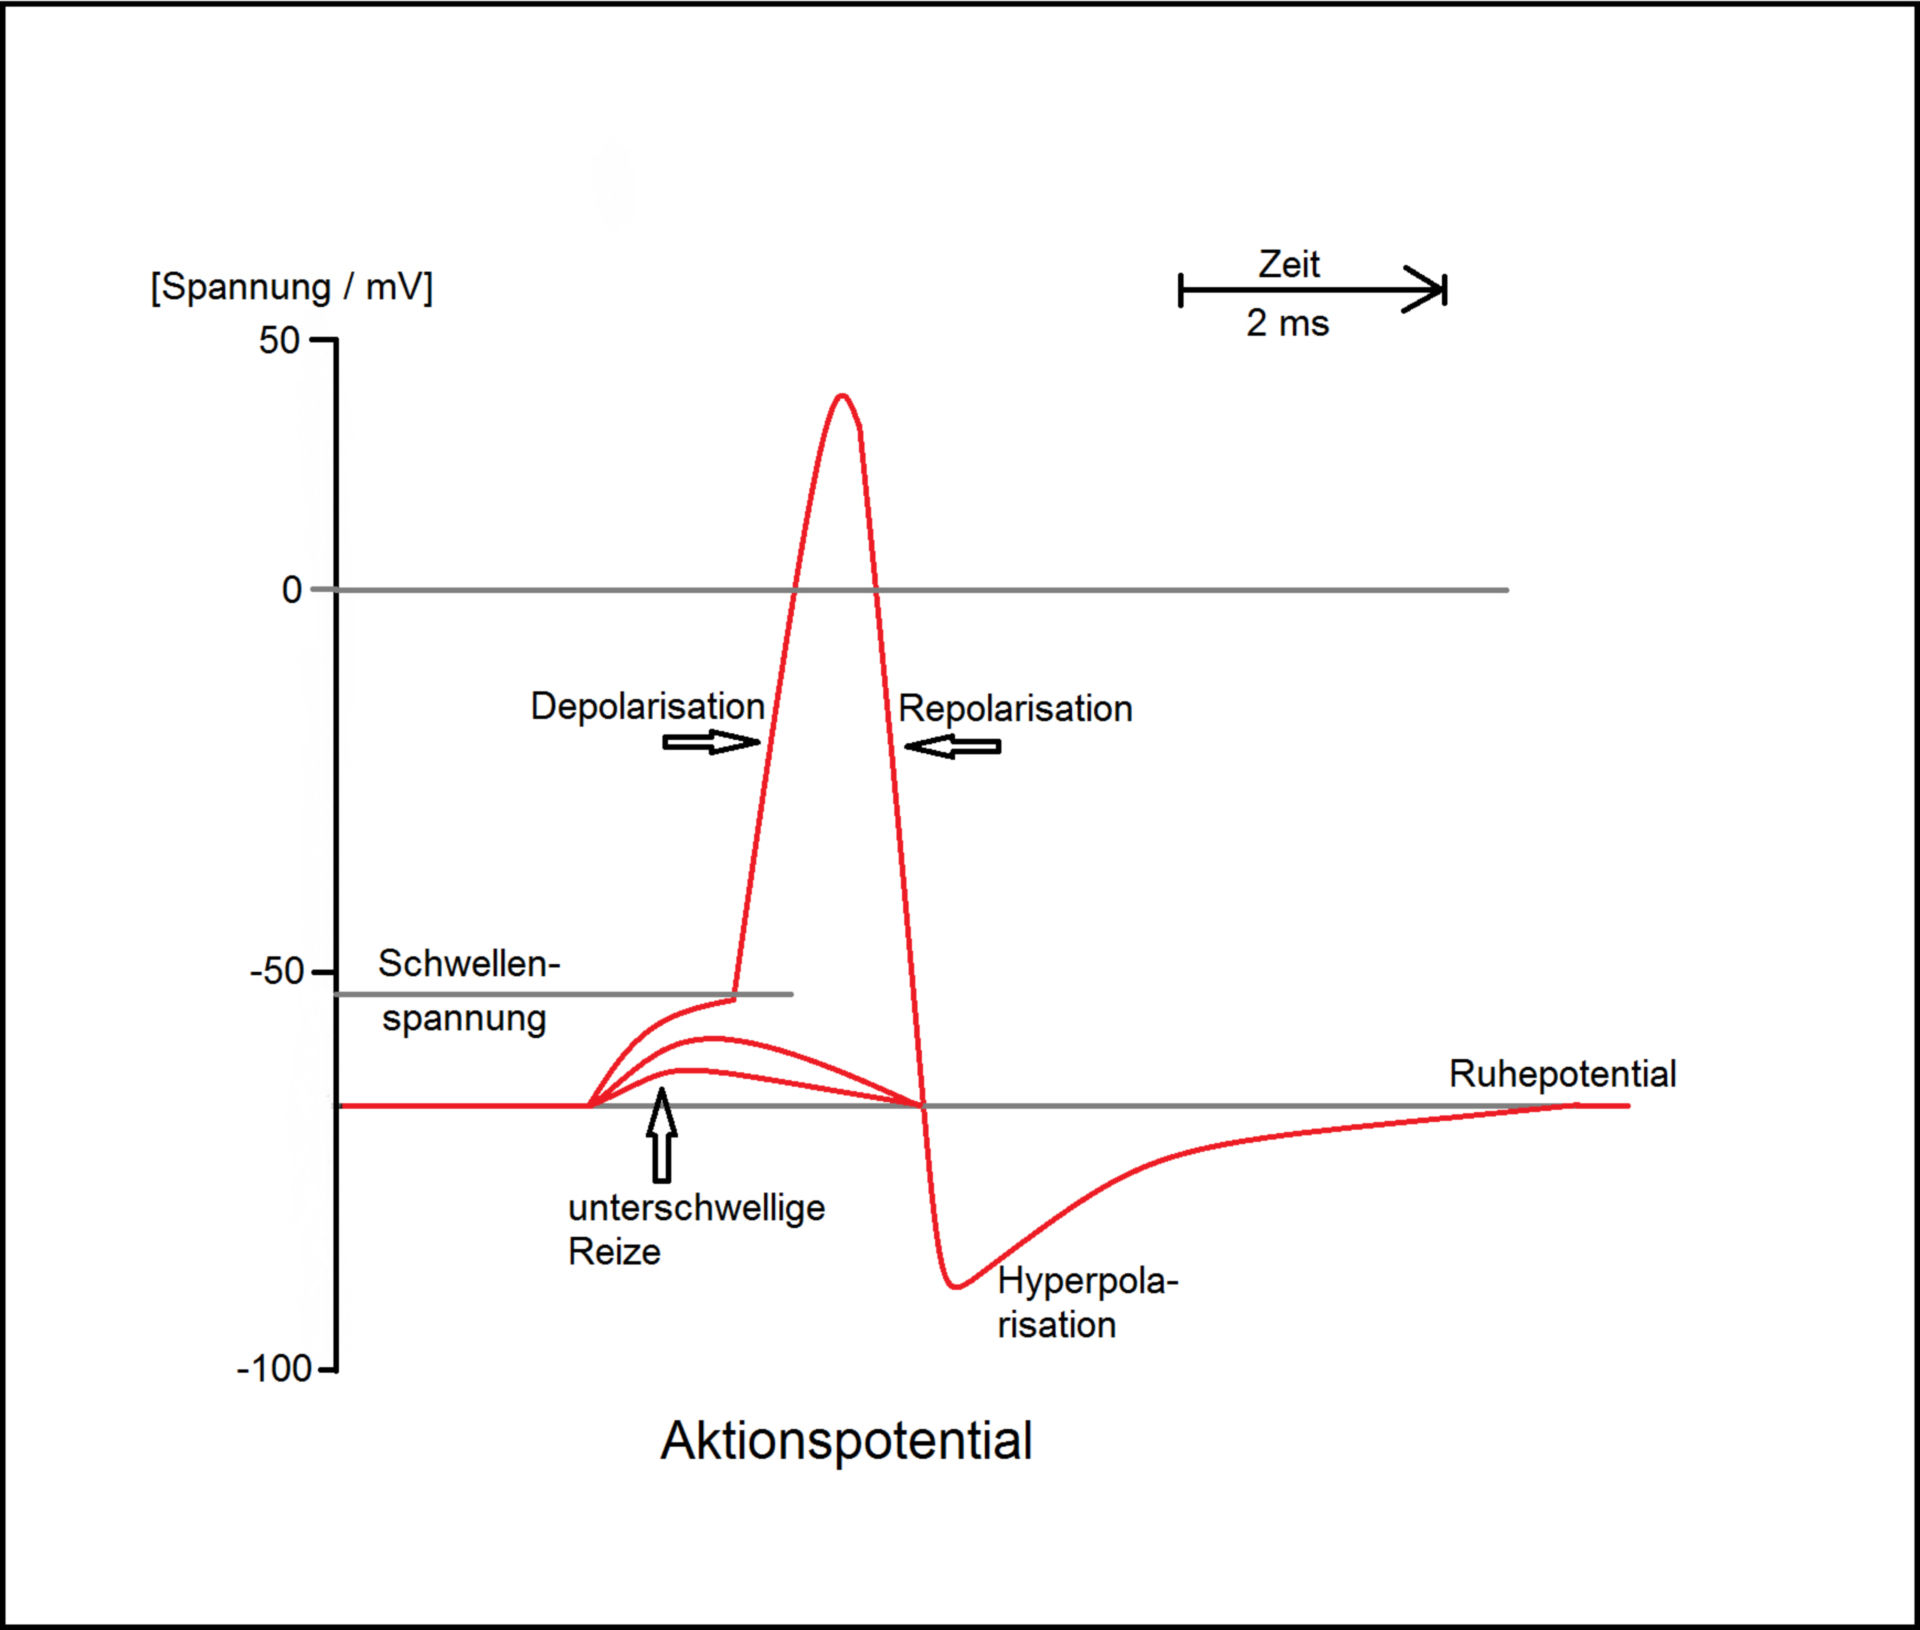
\includegraphics[width=0.8\textwidth]{abbildungen/APbild.jpg} % Lädt das Bild, skaliert es auf 80% der Textbreite
	\caption{UNterschrift nötig \parencite{DocCheckAPBIld}
	} % Die Bildunterschrift
	\label{fig:APbild} % Ein Label für Querverweise (z.B. "siehe Abbildung \ref{fig:beispielbild}")
\end{figure}

Das Aktionspotential breitet sich anschließend entlang des Axons aus.
Das Axon ist häufig von einer Myelinscheide umgeben, die von spezialisierten Gliazellen gebildet wird. Die Myelinscheide dient als elektrische Isolierung und ist in
regelmäßigen Abständen durch Ranvier-Schnürringe unterbrochen
(siehe Abbildung \ref{fig:salaNBG}). Die spannungsgesteuerten Natrium- und
Kaliumionenkanäle sind dabei überwiegend an den Ranvier-Schnürringen
konzentriert. Eine Depolarisation, die durch ein Aktionspotential an
einem Ranvier-Schnürring ausgelöst wurde, breitet sich im Zellplasma
aus und führt auch am nächsten Ranvier-Schnürring zur Öffnung
spannungsgesteuerter Natriumionenkanäle. Dort wird nach dem zuvor
beschriebenen Prinzip erneut ein Aktionspotential ausgelöst. Das Aktionspotential wird also durch die spannungsgesteuerten
Ionenkanäle sequenziell nur an den Ranvier-Schnürringen neu generiert und so entlang des Axons bis zu den
synaptischen Endigungen weitergeleitet, wobei die spannungsgesteuerten
Kaliumionenkanäle für die Repolarisation verantwortlich sind. Dies
bezeichnet man als saltatorische
Erregungsleitung.\footcite[S.~1090--1091]{Markl1997}

% ── Abbildung 3 ausgelassen ──────────────────────────────────
% Abbildung 3: Saltatorische Erregungsweiterleitung
% Quelle: \cite[S.~1091]{Markl1997}
% ─────────────────────────────────────────────────────────────
\begin{figure}[h] % [h] versucht, das Bild hier zu platzieren (hier), [t] für oben, [b] für unten
	\centering % Zentriert das Bild horizontal
	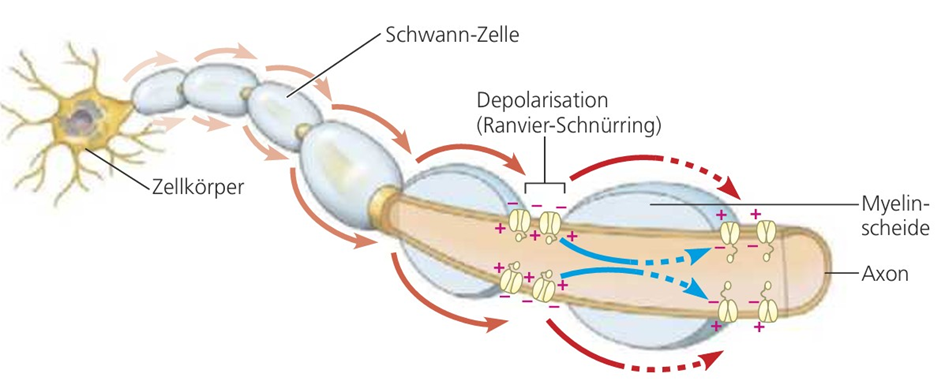
\includegraphics[width=0.8\textwidth]{abbildungen/SaltatorischeNBG.png} % Lädt das Bild, skaliert es auf 80% der Textbreite
	\caption{Saltatorische Erregungsweiterleitung \parencite{MarklBild1997b}
	} % Die Bildunterschrift
	\label{fig:salaNBG} % Ein Label für Querverweise (z.B. "siehe Abbildung \ref{fig:beispielbild}")
\end{figure}


Trifft ein Aktionspotential an der präsynaptischen Endigung ein, kommt
es zur Depolarisation der Membran, was zur Öffnung
spannungsgesteuerter Calciumionenkanäle führt. Der folgende Einstrom von
Calciumionen führt zur Fusion der synaptischen Vesikel mit der Membran
und zur Freisetzung von Neurotransmittern in den synaptischen Spalt. (siehe Abbildung 2.4)
\clearpage

% ── Abbildung 4 ausgelassen ──────────────────────────────────
% Abbildung 4: Aufbau und Funktionsweise einer chemischen Synapse
% Quelle: \cite{DocCheckSynapse2026}
% ─────────────────────────────────────────────────────────────
\begin{figure}[h] % [h] versucht, das Bild hier zu platzieren (hier), [t] für oben, [b] für unten
	\centering % Zentriert das Bild horizontal
	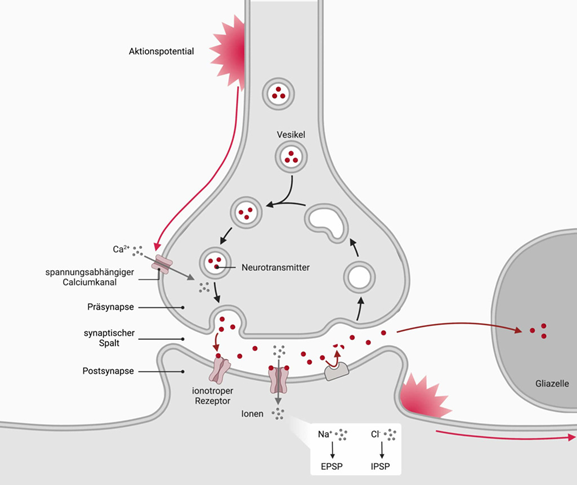
\includegraphics[width=0.7\textwidth]{abbildungen/chemsynapseNBG.png} % Lädt das Bild, skaliert es auf 80% der Textbreite
	\caption{Aufbau und Funktionsweise einer chemischen Synapse \parencite{DocCheckSynapseBild2026}
	} % Die Bildunterschrift
	\label{fig:chemNNBG} % Ein Label für Querverweise (z.B. "siehe Abbildung \ref{fig:beispielbild}")
\end{figure}

Spannungsabhängige Kaliumionenkanäle des Typs Kv1 spielen eine wichtige
Rolle bei der Repolarisation der Membran. Sie begrenzen auch hier die
Dauer des Aktionspotentials und dadurch den Calciumioneneinstrom. So
beeinflussen sie indirekt die Menge an freigesetzten Neurotransmittern.
Je nach Art der freigesetzten Neurotransmitter unterscheidet man
erregende und hemmende Synapsen. Zum Beispiel ist Glutamat ein wichtiger
erregender (exzitatorischer) Transmitter. Für den Transport von Glutamat
in die synaptischen Vesikel ist das Vesikelprotein VGlut1 (Vesikulärer
Glutamat-Transporter~1) verantwortlich. Daher dient VGlut1 als Marker
für exzitatorische Synapsen. Das Protein VGat (Vesikulärer
GABA/Glyzin-Transporter) hingegen transportiert inhibitorische
Neurotransmitter wie Gammaaminobuttersäure (GABA) in die Vesikel und ist
somit ein Marker für hemmende
Synapsen.\footcite[S.~1092]{Markl1997}

% ── Abbildung 6 ausgelassen ──────────────────────────────────
% Abbildung 6: Domänenorganisation von Caspr2
% Quelle: \cite{Canali2018}
% ─────────────────────────────────────────────────────────────
\clearpage
\section{Immunologische Grundlagen}
\textbf{Kushagr Sinha}

%Bei den autoimmunen Enzephalitiden kann man schon am Namen erkennen, dass es sich hier um eine autoimmune Krankheit handelt. Was eine autoimmune Krankheit ist, wie diese entsteht sowie die wichtigsten Grundlagen dazu, werden in diesem Kapitel erklärt.

Bei den autoimmunen Enzephalitiden handelt es sich um entzündliche Erkrankungen des Gehirns, bei denen das Immunsystem fehlgeleitet ist und dadurch körpereigene Stoffe angreift (= autoimmun). Um diese autoimmune Krankheit und ihre Entstehung zu verstehen, wird in diesem Kapitel zunächst auf die wichtigsten Grundlagen des gesunden und des fehlgeleiteten Immunsystems eingegangen.
\subsection{Prinzipien der Immunabwehr}

Das Immunsystem des menschlichen Körpers ist ebenso wie das Nervensystem äußerst komplex. Seine Hauptaufgabe besteht darin, den Körper vor Viren, Bakterien und anderen körperfremden Stoffen zu schützen.\footcite{Smith1999}\\

Außerdem wird das Immunsystem in zwei Systeme unterteilt:
\begin{itemize}
	\item das angeborene (unspezifische) Immunsystem
	\item das adaptive (spezifische) Immunsystem
\end{itemize}

Das angeborene Immunsystem wirkt im Falle eines Krankheitserregers als erstes, am schnellsten und unspezifisch, also ohne Erkennung spezifischer Antigene, indem es auf allgemein charakteristische Strukturen der Erreger reagiert.\footcite{MSDImmunsystem2026}

Das adaptive Immunsystem hingegen reagiert langsamer als das angeborene, wirkt aber spezifisch gegen die Antigene der Erreger. Außerdem bildet es ein immunologisches Gedächtnis, um beim Wiederauftreten des Pathogens dieses schneller und besser bekämpfen zu können. Die zwei wichtigsten Zellen dabei sind die T-Lymphozyten und die B-Lymphozyten.\footcite{MSDImmunsystem2026}

T-Lymphozyten übernehmen vorwiegend regulatorische und zellvermittelte Funktionen. T-Helferzellen koordinieren die Immunantwort, indem sie durch die Ausschüttung von Zytokinen die Aktivierung anderer Immunzellen steuern. Zytotoxische T-Zellen sind hingegen in der Lage, virusinfizierte oder entartete Körperzellen gezielt zu zerstören. Die präzise Zusammenarbeit dieser verschiedenen Zelltypen ermöglicht eine effektive und kontrollierte Immunabwehr.

%B-Lymphozyten spielen eine entscheidende Rolle bei der humoralen Immunantwort. Nach Aktivierung durch Antigenkontakt und Unterstützung durch T-Helferzellen differenzieren sie sich zu Plasmazellen, die große Mengen spezifischer Antikörper produzieren. Antikörper sind Proteine, die meist der Klasse der Immunglobuline G (IgG) angehören und eine charakteristische Y-förmige Struktur besitzen (siehe Abbildung \ref{fig:yfigure}). Die variablen Regionen an den Enden der Antikörper ermöglichen eine hochspezifische Bindung an Antigene. Durch diese Bindung können Krankheitserreger neutralisiert oder für andere Immunzellen markiert werden.\footcite{DocCheckLymphozyt, doccheck_igg}

B-Lymphozyten differenzieren sich nach Aktivierung durch Antigenkontakt und Unterstützung durch T-Helferzellen zu Plasmazellen, welche große Mengen spezifischer Antikörper produzieren. Antikörper sind Proteine, die meist der Klasse der Immunglobuline G (IgG) angehören und eine charakteristische Y-förmige Struktur besitzen (siehe Abbildung \ref{fig:yfigure}). Die variablen Regionen an den Enden der Antikörper ermöglichen eine hochspezifische Bindung an Antigene. Durch diese Bindung können Krankheitserreger neutralisiert oder für andere Immunzellen markiert werden.\footcite{DocCheckLymphozyt, doccheck_igg}


\begin{figure}[h] % [h] versucht, das Bild hier zu platzieren (hier), [t] für oben, [b] für unten
	\centering % Zentriert das Bild horizontal
	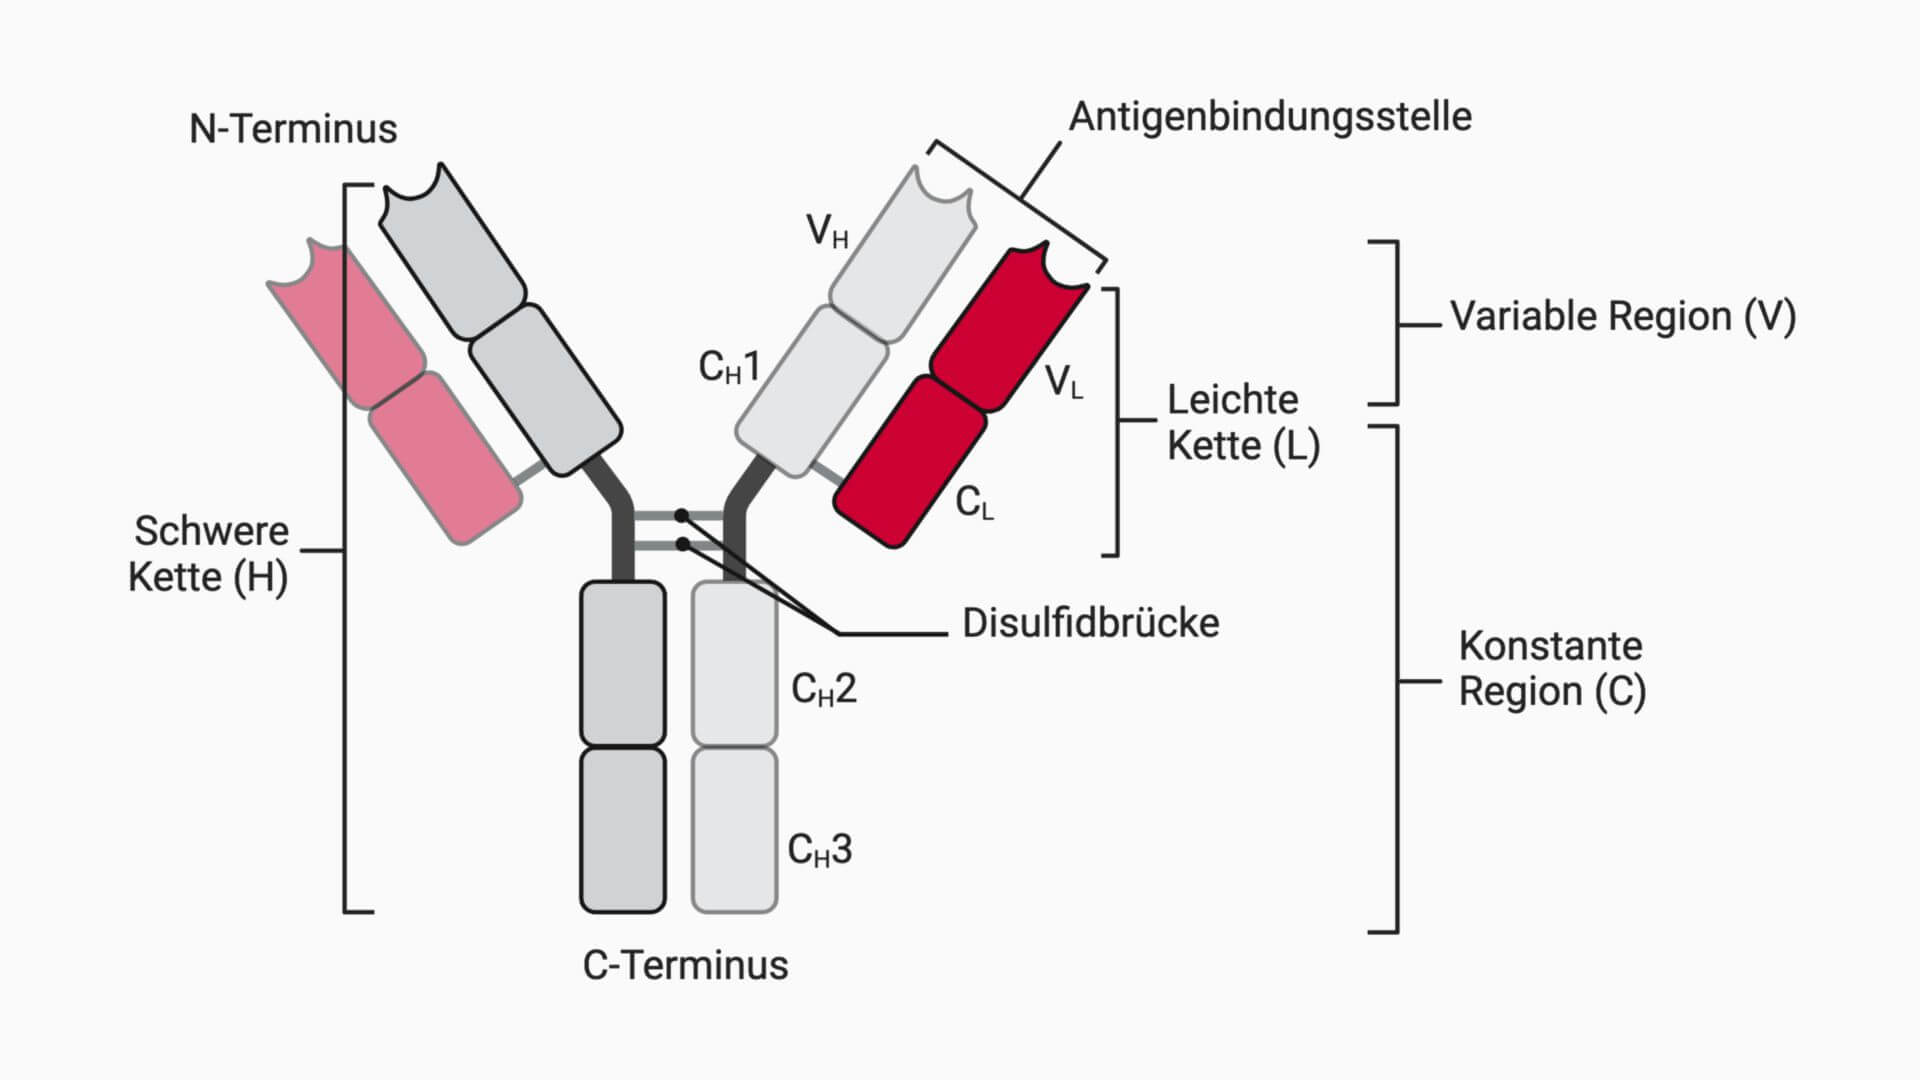
\includegraphics[width=0.91\textwidth]{abbildungen/IGGPI.jpg} % Lädt das Bild, skaliert es auf 80% der Textbreite
	\caption{Darstellung eines IgG-Antikörpers mit Beschriftung der strukturellen Regionen. \parencite{IGGbild_4u}} % Die Bildunterschrift
	\label{fig:yfigure} % Ein Label für Querverweise (z. B. "siehe Abbildung \ref{fig:beispielbild}")
\end{figure}

Damit beide Systeme miteinander kommunizieren können, gibt es dendritische Zellen. Diese gelten als Vermittler zwischen dem angeborenen und dem adaptiven Immunsystem. Sie erfüllen diese Aufgabe, indem sie Antigeninformationen von Erregern aufnehmen und diese dann an ihrer Oberfläche präsentieren. Dadurch werden Lymphozyten aktiviert, was wiederum zu einer spezifischen Immunantwort führt.\footcite{UniHeidelbergImmunologie2026}

Die Immunglobulinklasse G (IgG) umfasst vier Subklassen (IgG1 bis IgG4), die sich in ihrer Funktion unterscheiden und in Abbildung \ref{fig:yfigure} dargestellt sind. Während IgG1 und IgG3 oft Entzündungen durch das sogenannte Komplementsystem verstärken, nimmt IgG4 eine Sonderrolle ein: Es ist weniger entzündlich, neigt aber dazu, Bindungen zwischen Proteinen direkt zu blockieren.\footcite{doccheck_igg, AntwerpesIgG4}


\subsection{Mechanismen fehlgeleiteter Immunabwehr}

Ein zentrales Merkmal eines funktionierenden Immunsystems ist die Fähigkeit zur Selbsttoleranz. Das bedeutet, dass körpereigene Strukturen unter normalen Bedingungen nicht als Ziel einer Immunreaktion erkannt werden. Diese Eigenschaft ist entscheidend, um autoimmune Prozesse zu verhindern.\footcite{Smith1999}

Passiert bei der immunologischen Selbsttoleranz ein Fehler, greift das Immunsystem fälschlicherweise körpereigene Strukturen an. Dieser Vorgang wird als Autoimmunität bezeichnet. Erst wenn eine solche Reaktion zu messbaren Schäden an Organen oder Geweben führt und klinische Symptome aufweist, spricht man von einer Autoimmunerkrankung.\footcite{Fernandez2026}

%T- und B-Zellen entstehen beide im Knochenmark, durchlaufen jedoch bei ihrer Entwicklung spezifische Kontrollmechanismen, um eine Autoimmunität zu verhindern. Sie durchlaufen zunächst im Thymus bzw. im Knochenmark eine zentrale Toleranz, bei der geprüft wird, ob sie auf körpereigene Antigene reagieren. Ist dies der Fall, werden sie eliminiert.\footcite{DocCheckLymphozyt}

T- und B-Zellen reifen aus Vorläuferzellen im Thymus (daher auch T-Zelle) beziehungsweise im Knochenmark (B für engl. Bone Marrow). Bei ihrer Entwicklung durchlaufen sie eine zentrale Toleranz, bei der geprüft wird, ob sie auf körpereigene Antigene reagieren. Ist dies der Fall, werden sie eliminiert. Damit wird eine Autoimmunität verhindert.\footcite{DocCheckImmuntoleranz, DocCheckLymphozyt}

%Versagen die Toleranzmechanismen oder machen sie einen Fehler, sodass ein selbstreaktiver Lymphozyt überlebt und autoaggressive T-Zellen sowie Autoantikörper bildet, greift ein zusätzlicher Regulationsprozess ein, nämlich die periphere Toleranz. Hierbei unterdrücken regulatorische T-Zellen mithilfe von hemmenden Botenstoffen die Aktivierung solcher schädlicher Zellen oder lösen ihren Zelltod aus. Darüber hinaus kann die Zelle, wenn keine Entzündung vorliegt und somit keine kostimulatorischen Signale erhält, in einen Zustand der Inaktivität (Anergie) versetzt werden und somit keine Reaktion auslösen.\footcite{Macian2004, DocCheckImmuntoleranz}

Zusätzlich gibt es noch einen Selektionsprozess, die periphere Toleranz. Hierbei werden die T-Zellen gegen weitere Antigene getestet, die z. B. im Blut oder in Lymphknoten vorkommen. Dabei unterdrücken regulatorische T-Zellen mithilfe von hemmenden Botenstoffen die Aktivierung schädlicher Zellen oder lösen ihren Zelltod aus. Darüber hinaus kann die Zelle, wenn keine Entzündung vorliegt und sie somit keine kostimulatorischen Signale erhält, in einen Zustand der Inaktivität versetzt werden und somit keine Reaktion auslösen.\footcite{Macian2004, DocCheckImmuntoleranz}


%Zentral für die Entstehung der CASPR2-Enzephalitis ist ein Versagen der immunologischen Kontrollmechanismen: Selbstreaktive B-Zellen bilden Autoantikörper, die überwiegend zur IgG4-Subklasse gehören. Diese Antikörper gelangen über die Blut-Hirn-Schranke, eine normalerweise selektive Barriere zwischen Blutkreislauf und Gehirn, die das Eindringen schädlicher Stoffe verhindert, in das zentrale Nervensystem. Dort richten sie sich gegen das Protein CASPR2. Da IgG4-Antikörper kaum entzündliche Reaktionen auslösen, kommt es nicht zu einer direkten Zerstörung von Nervengewebe. Stattdessen beeinträchtigen sie die Funktion der Nervenzellen, indem sie die Stabilität von Kaliumkanälen stören. Die Folge ist eine erhöhte neuronale Erregbarkeit, die charakteristisch für die Erkrankung ist.\footcite{Patterson2018}

Die beschriebenen Mechanismen der immunologischen Selbsttoleranz sind auch für das Verständnis der Caspr2-Enzephalitis relevant. Bei dieser Erkrankung richtet sich die Immunantwort gegen körpereigene Strukturen des Nervensystems, insbesondere gegen das Protein Caspr2. (Im weiteren Verlauf wird daher betrachtet, welche Rolle Autoantikörper gegen Caspr2 bei der Erkrankung spielen.)

\chapter{Die Wirkung von Caspr2 am Axon und der Synapse}
\textbf{Johanna Hoppe}

Bei der beschriebenen Form der Erregungsleitung entlang des Axons
spielen neben den spannungsgesteuerten Ionenkanälen (vgl. Kapitel 2.1.2) auch weitere Proteine eine entscheidende Rolle.

Bereits 1999 wurde das Protein Contactin-associated
protein~2 (Caspr2) in den angrenzenden Bereichen der axonalen Schnürringe, den
juxtaparanodalen Bereichen,
beschrieben\footcite{Poliak1999} und seitdem weiter erforscht. Caspr2
ist ein Typ-I-Transmembranprotein, also ein integrales Protein, welches
die Zellmembran nur einmal durchquert, und gehört zur
Neurexin-Superfamilie. Diese ist eine Gruppe von
Transmembranmolekülen, die Zell-Zell-Kontakte vermitteln und
spezialisierte membranöse Domänen
erzeugen. Caspr2 wiest eine charakteristische Domänenstruktur auf, die in Abbildung 3.2 Teil B dargestellt ist. Dazu gehören unter anderem die Discoidin-Domäne (F58C) und die Laminin-Domänen (L1--L4), welche in Kapitel 6 der Arbeit erneut aufgegriffen werden. \footcites{HaklaiTopper2010}{CellSignaling2026} 

Caspr2 ist am myelinisierten Axon unter anderem mit Contactin2
Bestandteil eines Proteinkomplexes, welcher in Abbildung \ref{fig:cmyelin} dargestellt
ist. Dieser lokalisiert und verankert spannungsgesteuerte
Kalium-Ionenkanäle des Typs Kv1 in der Axonmembran. Dabei interagiert
Caspr2 extrazellulär mit Contactin2, welches wie Caspr2 als
Zelladhäsionsprotein wirkt. Dadurch trägt der Komplex entscheidend zur
räumlichen Organisation der myelinisierten Axonmembran und zur
Aufrechterhaltung einer effizienten saltatorischen
Erregungsweiterleitung bei. (siehe Kapitel~2.1.2) Eine Störung dieser
Interaktion kann die korrekte Clusterbildung und somit die Funktion der
Kv1-Kanäle beeinträchtigen und zu neurologischen Symptomen ,wie in
Kapitel~4.1 beschrieben wird,
führen.\footcite{VanSonderenNatRev2016}
\clearpage
% ── Abbildung 5 ausgelassen ──────────────────────────────────
% Abbildung 5: Caspr2 am myelinisierten Axon - BILD MIT BESSERER QUALI VON SELL EINFÜGEN
% Quelle: \cite{VanSonderenNatRev2016}
% ─────────────────────────────────────────────────────────────
\begin{figure}[h] % [h] versucht, das Bild hier zu platzieren (hier), [t] für oben, [b] für unten
	\centering % Zentriert das Bild horizontal
	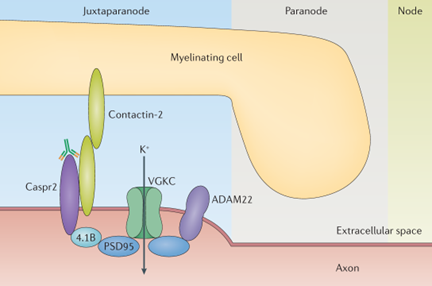
\includegraphics[width=0.91\textwidth]{abbildungen/caspr2myelinWCA.png} % Lädt das Bild, skaliert es auf 80% der Textbreite
	\caption{  Caspr2 am myelinisierten Axon \parencite{SonderenBild2017}} % Die Bildunterschrift
	\label{fig:cmyelin} % Ein Label für Querverweise (z.B. "siehe Abbildung \ref{fig:beispielbild}")
\end{figure}

Zudem ist bekannt, dass Caspr2 während der Embryonalentwicklung
bedeutsam ist und dort für die korrekte Verzweigung der Dendriten, die
Ausbildung dendritischer Spines und das Axonwachstum mitverantwortlich
ist. Fehlt Caspr2 durch eine genetische Veränderung, kann die
Entwicklung der Nervenzellen beeinträchtigt sein. Eine Caspr2-Mutation
wird beispielsweise auch mit Erkrankungen wie der
Autismus-Spektrum-Störung oder Aufmerksamkeits-/Hyperaktivitätsstörung
(ADHS) in Verbindung
gebracht.\footcite{Canali2018}

Neuere Studien zeigen, dass Caspr2 nicht nur am Axon lokalisiert ist,
sondern auch an Synapsen vorkommt, was bisher jedoch deutlich weniger
erforscht ist. Kv1-Kanäle sind bereits sicher an den präsynaptischen
Membranen bekannt und sind dort an der Freisetzung von
Neurotransmittern beteiligt (siehe Kapitel~2.1.2). Bereits 2008 konnten
Caspr2 und Contactin-2 biochemisch an synaptischen Membranen
nachgewiesen werden.\footcite{Bakkaloglu2008}
In einer weiteren Studie aus dem Jahr 2015 wurde mithilfe von
Immunfärbungen eine Überlappung von Caspr2 mit synaptischen Markern
erregender und hemmender Synapsen gezeigt. Dabei wurden die Marker
VGlut für exzitatorische, und Gad65 für inhibitorische Synapsen,
verwendet. Diese gelten als spezifische Markerproteine für den
jeweiligen Synapsentyp. Unter anderem durch solche Ergebnisse wird davon ausgegangen, dass Caspr2 auch an präsynaptischen Membranen
vorliegt.\footcite{Pinatel2015}

Die Funktion von Caspr2 an der Synapse ist bislang nicht vollständig
geklärt, ähnelt jedoch vermutlich der am Axon. Caspr2 bildet auch hier
einen Protein-Komplex mit weiteren Molekülen wie Contactin-2. Wie
dieser genau aufgebaut ist, ist jedoch noch unklar. Angenommen wird,
dass dieser Komplex analog zum myelinisierten Axon die Kv1-Kanäle
stabilisiert und lokalisiert. Darüber hinaus könnte der
Caspr2-Contactin-2-Komplex an der Organisation synaptischer Strukturen
beteiligt sein, indem er die Verbindung von Prä- und Postsynapse
stabilisiert. Die Anordnung des Proteinkomplexes sowie die Organisation
der einzelnen Domänen von Caspr2 ist wahrscheinlich eine andere als am
Axon, da es sich hier um andere Zellbereiche handelt. Weiterhin ist zu
beachten, dass der synaptische Spalt kleiner ist als der extrazelluläre
Raum zwischen Axon und Gliazelle. Entsprechend existieren
unterschiedliche Hypothesen zur Organisation und Funktion von Caspr2 an
der Synapse.\footcite{Canali2018} Teil~C der Abbildung \ref{fig:domänenc}  veranschaulicht zwei mögliche Anordnungen des Proteins an der Synapse:
zum einen eine vertikale Orientierung, die das Protein annehmen könnte,
sowie eine mögliche horizontale Orientierung der Domänen. Je nachdem,
wie das Protein ausgerichtet ist, wird seine Funktion unterschiedlich
beeinflusst, da beispielsweise andere Interaktionen mit weiteren
Proteinen möglich sind.\footcite{Canali2018}
% ── Abbildung 6 ausgelassen ──────────────────────────────────
% Abbildung 6: Domänenorganisation von Caspr2 A ABSCHNEIDEN
% Quelle: \cite{Canali2018}
% ─────────────────────────────────────────────────────────────
\begin{figure}[h] % [h] versucht, das Bild hier zu platzieren (hier), [t] für oben, [b] für unten
	\centering % Zentriert das Bild horizontal
	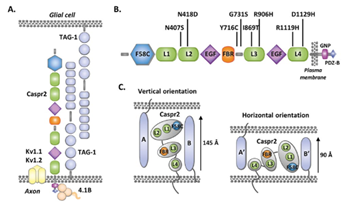
\includegraphics[width=0.91\textwidth]{abbildungen/Domänencaspr2WCA.png} % Lädt das Bild, skaliert es auf 80% der Textbreite
	\caption{Domänenorganisation von Caspr2 \parencite{CanaliBild2018}} % Die Bildunterschrift
	\label{fig:domänenc} % Ein Label für Querverweise (z.B. "siehe Abbildung \ref{fig:beispielbild}")
\end{figure}
\chapter{Autoimmune Enzephalitis und CASPR2}
\textbf{Helene Becker}
\section{Definition und Krankheitsbild}
Als Enzephalitis wird eine Entzündung des Gehirns bezeichnet.
Je nach Ursache und Ausprägung der Symptome werden verschiedene Arten
von Enzephalitiden unterschieden.

Enzephalitiden werden meist ausgelöst, indem ein Virus das Hirn direkt
infiziert oder ein Virus, ein Impfstoff oder etwas anderes die Entzündung
auslöst. Als Folge einer Viruserkrankung kann so beispielsweise eine
epidemische oder eine sporadische Enzephalitis entstehen. Ebenfalls kann
(aus einer Virusinfektion oder aus der Reaktion von T-Zellen auf einen Tumor) eine 
autoimmune Enzephalitis (AE) hervorgehen.\footcite{Klein2026}
Bei der AE handelt es sich um eine Autoimmunerkrankung, bei der es zur
fehlgeleiteten Immunabwehr gegen körpereigene neuronale Strukturen
kommt.\footcites{Klein2026}{Fernandez2026}
Dabei werden AK gegen Antigene körpereigener Gewebe durch das
Immunsystem hergestellt, jene werden dann als sogenannte aAK
bezeichnet. Eine solche Autoimmunreaktion kann zu neuronalen 
Entzündungen und Gewebeschäden führen.\footcite{Fernandez2026}

Der Begriff AE beschreibt eine Gruppe von Erkrankungen, die sich in verschiedenen Bereichen des
ZNS und PNS ausbilden. Jede
einzelne wird an Hand der auslösenden aAK charakterisiert, die sich gegen bestimmte neuronale Strukturen bzw. 
Antigene richten. Durch die vielfältigen Antigene gibt es
ein breites Spektrum klinischer Symptome der AE, die von
Wesensänderungen und kognitiven Störungen über epileptische Anfälle und
Bewegungsstörungen bis hin zu vegetativen und Bewusstseinsstörungen
reichen können.\footcite[S.~525]{Heine2022}


Sporadische AE werden in zwei Hauptformen unterschieden. Paraneoplastische
Enzephalitiden werden durch aAK, sogenannte onkoneurale AK, gegen
intrazelluläre Zielstrukturen (siehe Abbildung \ref{fig:AE2} A) ausgelöst und sind meist Tumor-assoziiert.
\\
%neues Bild ans ende des Absatzes!! Quelle: https://epub.jku.at/download/pdf/7708824 => Abbildung 3 Seite 12; Bildunterschrift: A: onkoneurale AK richten sich gegen intrazelluläre Proteine. B: aAK gegen neuronale Oberflächenantigene.  !! die andere Abbildung muss dann umbenannt werden
\\
AAK gegen neuronale Oberflächenantigene (siehe Abbildung \ref{fig:AE2} B) lösen eine sogenannte
nicht-paraneoplastische Enzephalitis und sind eher selten mit
Tumoren assoziiert. Eines dieser neuronalen Oberflächenantigene ist
Caspr2.\footcite[S.~526--528]{Heine2022}

\begin{figure}[h] % [h] versucht, das Bild hier zu platzieren (hier), [t] für oben, [b] für unten
	\centering % Zentriert das Bild horizontal
	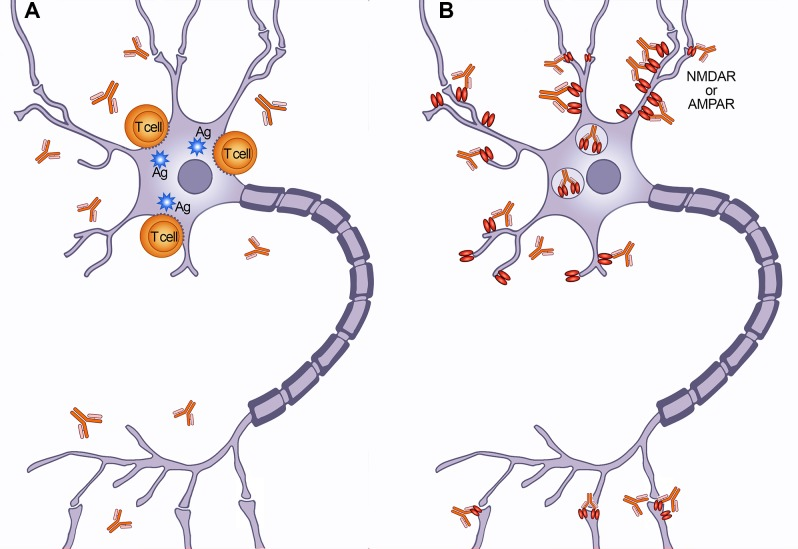
\includegraphics[width=0.85\textwidth]{abbildungen/AE2Bild.jpg} % Lädt das Bild, skaliert es auf 80% der Textbreite
	\caption{ A: onkoneurale AK richten sich gegen intrazelluläre Proteine. B: aAK gegen neuronale Oberflächenantigene. \parencite{PNSChannelBild2017}} % Die Bildunterschrift
	\label{fig:AE2} % Ein Label für Querverweise (z.B. "siehe Abbildung \ref{fig:beispielbild}")
\end{figure}

Generell verlaufen AE in der Regel zunächst subakut bis chronisch. Über
den Langzeitverlauf von AE wurden bisher nur wenige Daten erhoben. Je
nach Zeitpunkt der Diagnosestellung und des Therapiebeginns kommt es bei
nicht-paraneoplastischen AE allerdings meist zur vollständigen oder
teilweisen Erholung.\footcite[S.~533]{Heine2022}
Kurz nach der Akutphase sind die Genesungschancen für Patienten zwar am
höchsten, dennoch lassen sich noch nach mehreren Jahren Verbesserungen
der kognitiven Fähigkeiten
verzeichnen.\footcite[S.~534]{Heine2022}
Paraneoplastische Enzephalitiden hingegen sind meist Tumor-assoziiert,
sprechen daher selten auf immunwirksame Behandlungen an und erzeugen oft
schwere und bleibende neurologische
Ausfallerscheinungen.\footcite{UniHeidelbergAE2026}

Da sich diese Arbeit mit der Caspr2-AE auseinandersetzt, ist
im Folgenden zunächst von nicht-paraneoplastischen Enzephalitiden
die Rede.

Zur Diagnostik einer AE hilft die Zuordnung erhobener Befunde in Kategorien. Diese Befunde stammen unter anderem aus der
klinischen Analyse der Symptome und möglicher Syndrome,
Magnetresonanztomographie (MRT), Liquoranalyse,
Elektroenzephalogramm (EEG) und Antikörperdiagnostik. In Graus et al.\ (2016) findet sich ein klinischen Diagnosealgorithmus, der ausgehend vom Verdacht auf eine autoimmune Enzephalitis verschiedene klinisch charakterisierbare Syndrome, sowie antikörperassoziierte und antikörpernegative Erkrankungen berücksichtigt.
\footcite[S.~394]{Graus2016}

Wie in Abbildung \ref{fig:AE1} zu erkennen ist, sollte bei Verdacht einer AE eine Diagnostik 
auf zugrundeliegende aAK initiiert werden. Dies
sollte in Abhängigkeit von klinischen Syndromen und Zusatzbefunden (siehe oben) geschehen. Zwar
kann die Diagnose einer AE ohne Nachweis von AK bei AE-typischen
Veränderungen im Liquor, MRT und EEG sowie dem zusätzlichen Ausschluss
wichtiger Differentialdiagnosen gestellt werden, allerdings führt erst
der Nachweis von aAK zu einer sicheren
Diagnose.\footcites[S.~394]{Graus2016}{GenerateNet2026}

\begin{figure}[h] % [h] versucht, das Bild hier zu platzieren (hier), [t] für oben, [b] für unten
	\centering % Zentriert das Bild horizontal
	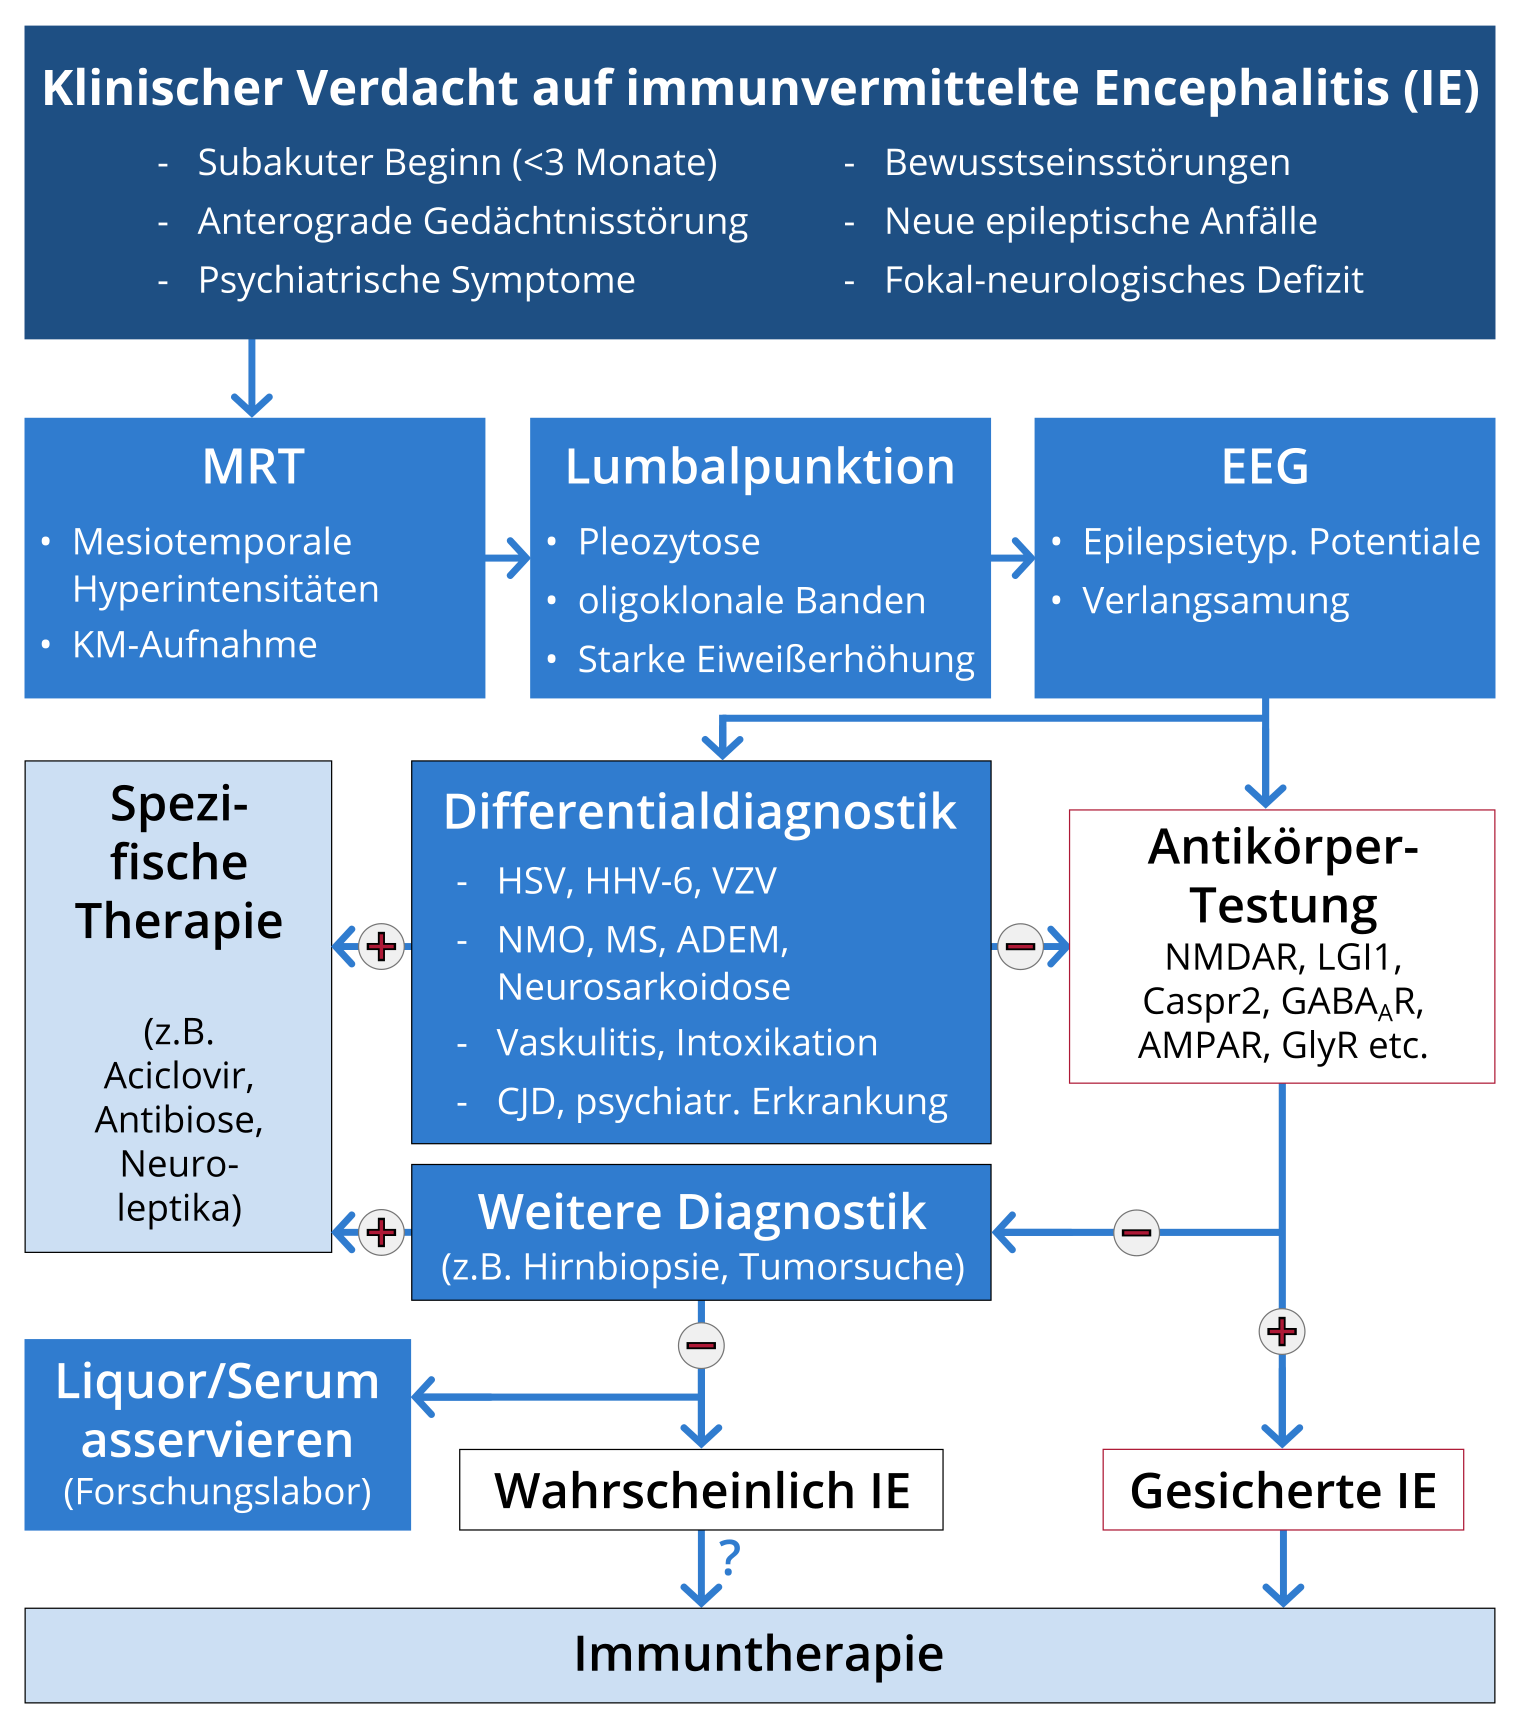
\includegraphics[width=0.85\textwidth]{AE1bild.png} % Lädt das Bild, skaliert es auf 80% der Textbreite
	\caption{ Vereinfachter schematischer Ablauf der Diagnose und
		Differentialdiagnose autoimmuner
		Enzephalitiden. \parencite{GenerateNetBild2026}} % Die Bildunterschrift
	\label{fig:AE1} % Ein Label für Querverweise (z.B. "siehe Abbildung \ref{fig:beispielbild}")
\end{figure}

\clearpage
Die Therapie von AE sollte auch ohne bestätigten Antikörpernachweis
frühestmöglich beginnen, um die weitere Entzündung des Gehirns durch das
Immunsystem zu verhindern. Dabei ist die Therapie in zwei Bereiche mit
verschiedenen Therapiemöglichkeiten unterteilt. Die Erstlinientherapie,
bspw.\ mit hochdosierten Steroiden, dient zunächst der Abschwächung der
Immunreaktion. Um die Erkrankung langfristig unter Kontrolle zu bekommen, ist eine
weitere Therapie mit Medikamenten, die gezielt AK-produzierende B-Zellen beseitigen,
sinnvoll. Zusätzlich zu einer Immuntherapie erfolgt meist eine
symptomatische Behandlung. Im Falle von Tumoren müssen diese zunächst entfernt oder behandelt werden. 
Es werden ebenfalls nichtmedikamentöse
Maßnahmen, wie Physiotherapie oder neurologische Rehabilitation, zur
Förderung der funktionalen Fähigkeiten, die zuvor durch die AE gemindert wurden, im Alltag
angeraten.\footcite[S.~533]{Heine2022}
Einerseits, weil sich bei einzelnen AE auch nach mehreren Jahren
Verbesserungen von kognitiven Funktionen erkennen
lassen\footcite[S.~534]{Heine2022}, andererseits weil selbst nach einer
Verbesserung der Symptomatik ein Rückfall nicht auszuschließen
ist.\footcite[S.~11]{Lancaster2015}


AE werden nach den auslösenden aAK charakterisiert und benannt. Die
Caspr2-Enzephalitis wird durch die anti-Caspr2-aAK ausgelöst. Sie geht
häufig einher mit bestimmten Symptomen und Syndromen, die jedoch von
Patient zu Patient variieren.\footcite[S.~525--526]{VanSonderen2016}

Dazu zählen:
\begin{itemize}
	\item Übererregbarkeit des PNS:
	\begin{itemize}
		\item Neuromyotonie (Die Überaktivität der Nerven, welche die Muskelfasern anregen. Es entwickelt sich eine fortschreitende Versteifung der Muskeln, ein anhaltendes Muskelzittern sowie Zuckungen und Krämpfe.)\footcite{MSDNeuromyothonie2024}
		\item neuropathische Schmerzen, sowie Gelenk-, Muskel- und
		Brustschmerzen
	\end{itemize}
	\item limbische Enzephalitis
	\item Morvan-Syndrom (Kombination aus neuropsychiatrischen Symptomen
	[Schlafstörung, kognitive Defizite], autonomer
	Funktionsstörung [Störung von unwillkürlichen Körperprozessen, wie Herzschlag] und Neuromyotonie)
	\item Gewichtsverlust\footcites[S.~523; 526]{VanSonderen2016}%
	[S.~527; 530]{Heine2022}
\end{itemize}

Die meisten nicht-paraneoplastischen AE gehen deutlich seltener mit
Tumoren einher als paraneoplastische AE, so auch die
Caspr2-Enzephalitis. Ist dies dennoch der Fall, dann handelt es sich
meist um Tumore der Thymusdrüse.\footcite[S.~527; 530]{Heine2022}

Es lässt sich feststellen, dass überwiegend ältere Männer von der
Caspr2-Enzephalitis betroffen sind, wobei das durchschnittliche Alter zum
Zeitpunkt des Auftretens der Symptome 66~Jahre
betrug.\footcite[S.~522--523; 526]{VanSonderen2016}

\section{Wirkungsweise der Anti-Caspr2-Autoantikörper}

Die Anti-Caspr2-aAK binden an die
extrazellulären Domänen von Caspr2 auf der Oberfläche von Nervenzellen.
Sie binden insbesondere an die Discoidin- und
Laminin-1-Domänen.\footcite[S.~6]{Olsen2015}

AK werden im Allgemeinen je nach ihrer Effektorfunktion in vier
Immunglobulin-Subklassen (IgG1--4)
unterschieden.\footcite{Mitrevski}
Die AK der Klasse IgG4 lösen kaum Entzündungsreaktionen aus, sondern
blockieren die Funktionen der Zielstrukturen, sodass beispielsweise die
Bindung von Antigenen an andere Antigene verhindert
wird.\footcite{AntwerpesIgG4}
Die IgG1-AK sind mit verstärkten Entzündungsreaktionen und
Komplementaktivierung assoziiert.\footcite{Mitrevski}
Der Test auf IgG4 ist in der Studie von van~Sonderen et~al.\ (2016) in
100\,\% der Fälle, in denen die Caspr2-Enzephalitis auftrat, positiv
ausgefallen. 63\,\% der Testergebnisse lieferten ein positives Ergebnis
bei der IgG-Klasse IgG1. 19~Patientinnen und Patienten wurden bezüglich
der IgG-Klasse der AK getestet.\footcite[S.~524]{VanSonderen2016}

Die Rückfallquote scheint ebenfalls hoch zu sein. In der klinischen
Forschung von van~Sondern et~al.\ (2016) liegt sie bei 25\,\%, wobei die
Rückfälle bis zu sieben Jahren nach Auftreten der Erkrankung eingetreten
sind.\footcite[S.~524]{VanSonderen2016}
Dabei sind die Anti-Caspr2-aAK nicht für eine geminderte Expression von
Caspr2 an der Zelloberfläche verantwortlich. Caspr2 wird durch die aAK
funktionell blockiert, sodass es nicht mehr mit Contactin2 interagieren
kann.\footcite[S.~6--7]{Patterson2018}\\
\\
Die Kaliumkanäle (Kv1.1/1.2), die normalerweise durch den Komplex in den
juxtaparanodalen Regionen der Axone verankert sind, verlieren ihre
räumliche Organisation.\footcites{Mitrevski}[S.~8]{Patterson2018}\\
\\
Wie in Kapitel~2.1.2 beschrieben, sind Kaliumkanäle für die
Repolarisation nach einem Aktionspotential essenziell. Bei gestörter
Verankerung kommt es zu axonaler Hyperexzitabilität, die Neuronen werden
also zu lange
erregt.\footcite[S.~525--526]{VanSonderen2016}
Dies erklärt die Symptome Neuromyotonie, Übererregbarkeit und
neuropathische Schmerzen aus Kapitel~4.1. Während die axonale Pathophysiologie gut verstanden ist,
ist die Wirkung von Anti-Caspr2-aAK an den Synapsen noch wenig
charakterisiert.

\chapter{Material und methodisches Vorgehen}
\textbf{Johanna Hoppe}
\section{Erklärung der Methode}

Indirekte Immunfluoreszenz
Ein zentrales Verfahren dieser Arbeit ist die
Immunhistochemie. Dies ist eine histologische Methode, mit der
spezifische Zellstrukturen, beispielsweise Proteine, sichtbar gemacht
werden. Diese Markierung basiert auf der Bindung von Antikörpern an ihre
Zielstruktur und somit auf der Antigen-Antikörper-Reaktion (siehe
Kapitel~2.2). Eine spezielle Form der Immunhistochemie ist die
Immunfluoreszenz mit indirekten Färbungen, welche in den folgenden
Untersuchungen verwendet wird.\footcite{LeicaIHC2026}

Im ersten Schritt der immunhistologischen Färbung wird ein
Primärantikörper auf die Zellstrukturen gegeben. Dieser bindet
spezifisch an das Zielantigen (siehe Abbildung \ref{fig:immnuofMMV}). Dabei unterscheidet man
zwischen polyklonalen und monoklonalen Antikörpern. Polyklonale
Antikörper binden an verschiedene Epitope des Antigens, da sie eine
Mischung mehrerer Antikörper darstellen, während monoklonale Antikörper
spezifisch an ein einzelnes Epitop binden. Sie werden von nur einer
Zelllinie produziert, die auf einen einzigen B-Lymphozyten
zurückgeht.\footcites{DocCheckMonoklonal}{DocCheckIHC}

Im nächsten Schritt bindet der Sekundärantikörper spezifisch an den
verwendeten Primärantikörper. Zudem ist dieser mit einem Farbstoff
gekoppelt, welcher unter dem Fluoreszenzmikroskop farbig sichtbar ist.
Daher spricht man von einem fluoreszenzbasierten Detektionssystem. Durch
den Nachweis des fluoreszierenden Antikörpers können somit die
untersuchten Proteine dargestellt und beispielsweise ihre Lokalisation
untersucht werden (siehe Abbildung \ref{fig:immnuofMMV}).\footcite{DocCheckIHC}
\clearpage
% ── Abbildung 7 ausgelassen ──────────────────────────────────
% Abbildung 7: Prinzip der indirekten Immunfluoreszenz BILD NOCH ZUSCHNEIDEN
% Quelle: \cite{LeicaMicrosystems2026}
% ─────────────────────────────────────────────────────────────
\begin{figure}[h] % [h] versucht, das Bild hier zu platzieren (hier), [t] für oben, [b] für unten
	\centering % Zentriert das Bild horizontal
	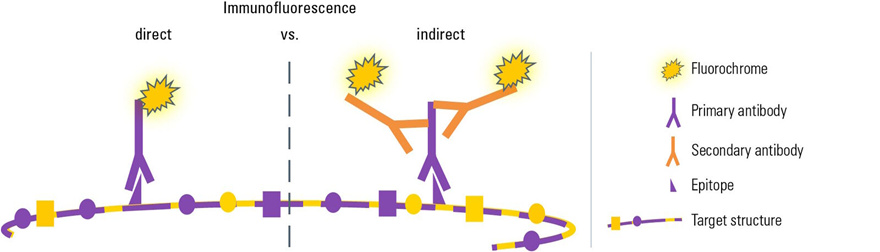
\includegraphics[width=0.91\textwidth]{abbildungen/immunoflurosenzMMV.png} % Lädt das Bild, skaliert es auf 80% der Textbreite
	\caption{ Prinzip der indirekten Immunfluoreszenz (rechts)\parencite{LeicaMicrosystems2026}} % Die Bildunterschrift
	\label{fig:immnuofMMV} % Ein Label für Querverweise (z.B. "siehe Abbildung \ref{fig:beispielbild}")
\end{figure}



Für optimale Färbungsergebnisse ist darauf zu achten, die Fixierung der
Zellen optimal sicherzustellen, geeignete Antikörper sorgfältig
auszuwählen und unspezifische Hintergrundfärbungen zu minimieren.
Letzteres wird unter anderem durch gründliche Waschschritte und
geeignete Blockierungsschritte erreicht. Zudem müssen Negativkontrollen
durchgeführt werden, um unspezifische Bindungen der Antikörper
auszuschließen. Auf diese Weise können die Auswertungen aussagekräftig
und präzise durchgeführt
werden.\footcite{LeicaIHC2026}

Um eine Kolokalisation zweier Proteine bei der mikroskopischen
Auswertung beurteilen zu können, müssen diese in einer Probe durch eine
Doppelfärbung sichtbar gemacht werden. Dazu werden zwei verschiedene,
jeweils proteinspezifische Primärantikörper eingesetzt. Dabei ist zu
beachten, dass diese aus zwei unterschiedlichen Spezies stammen. Für wissenschaftliche Zwecke werden die Antikörpern in Tieren generiert, indem sie das Antigen gespritzt bekommen, was eine gezielte Immunreaktion auslöst. Dadurch werden spezifische Antikörper produziert. Die
Sekundärantikörper sind jeweils spezifisch gegen die Spezies des
Primärantikörpers gerichtet, weshalb die Wahl von zwei
unterschiedlichen Spezies die eindeutige Zuordnung der Signale
ermöglicht und Kreuzreaktionen vermeidet. Zudem muss bei einer
Doppelfärbung beachtet werden, dass die an die Sekundärantikörper
gekoppelten Fluoreszenzfarbstoffe sich ausreichend unterscheiden, damit
es zu keiner Überlagerung der Signale kommt. Dies bedeutet, dass die
Spektren, in denen die Farbstoffe fluoreszieren, nicht stark überlappen
dürfen. Diese Spektren ergeben sich aus der jeweiligen Anregungs- und
Emissionswellenlänge.\footcite{Hackenberg}

Die Methode der indirekte Immunfluoreszenz wurde gewählt, da sie eine
Untersuchung der räumlichen Verteilung spezifischer Proteine innerhalb von
Nervenzellen ermöglicht. Dies ist für die vorliegenden Untersuchungen von
Bedeutung, da die Lokalisation von Proteinen an den synaptischen Strukturen
untersucht werden soll. Durch die Doppelfärbung von Caspr2 und den synaptischen
Markern VGlut und VGat beziehungsweise Contacin2 lässt sich feststellen, inwiefern
sich deren Signale räumlich überlagern. Auf diese Weise kann untersucht werden, ob
Caspr2 sowohl an erregenden als auch an hemmenden Synapsen lokalisiert ist und
ob Antikörper gegen Caspr2 die Kolokalisation von Caspr2 und Contacin-2
beeinflussen.

Mikroskopieverfahren 
Zur mikroskopischen Auswertung der Proben wurden die Methoden Widefield
Fluorescence Microscopy (WF) und Structured Illumination Microscopy (SIM)
angewendet.
Die Widefield Fluorescence Microscopy ist ein fluoreszenzmikroskopisches
Verfahren, bei dem das gesamte betrachtete Sichtfeld gleichzeitig mit Anregungslicht
beleuchtet wird. Dabei werden Fluorophore in der Probe durch Licht einer geeigneten
Wellenlänge angeregt. Nach der Anregung emittieren sie Licht mit einer anderen,
meist längeren Wellenlänge.
Eine zentrale Komponente der WF-Mikroskopie ist der dichroitische Spiegel (oder
Strahlteiler). Dieser befindet sich zwischen Lichtquelle und Mikroskopobjektiv und
erfüllt eine wichtige Trennfunktion. Das Anregungslicht wird vom Strahlteiler in
Richtung Probe reflektiert, während das von den Fluorophoren emittierte Licht den
Strahlteiler passieren kann. Die Eigenschaften des Strahlteilers müssen daher auf
die verwendeten Fluorophore abgestimmt sein, damit das Anregungslicht möglichst
effizient zur Probe gelangt und gleichzeitig das Fluoreszenzlicht zur Detektion
weitergeleitet wird. Das Mikroskopobjektiv wirkt zunächst als Kondensator und
fokussiert das Licht auf die Probe. Zudem sammelt es das von den Fluorophoren
ausgesendete Fluoreszenzlicht und bildet dieses auf einer Kamera ab.
\begin{figure}[h] % [h] versucht, das Bild hier zu platzieren (hier), [t] für oben, [b] für unten
	\centering % Zentriert das Bild horizontal
	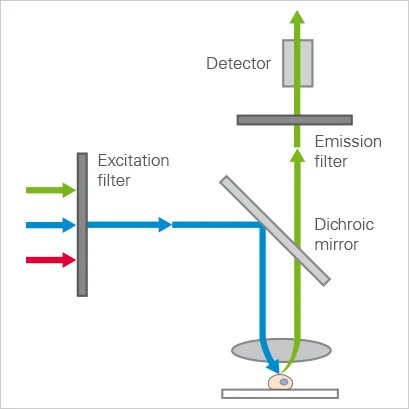
\includegraphics[width=0.91\textwidth]{abbildungen/WFMMV.jpg} % Lädt das Bild, skaliert es auf 80% der Textbreite
	\caption{ muss noch was sagen \parencite{ibidiWFMBild}} % Die Bildunterschrift
	\label{fig:WFBild} % Ein Label für Querverweise (z.B. "siehe Abbildung \ref{fig:beispielbild}")
\end{figure}
Die Structured Illumination Microscopy (SIM) ist eine Methode der
Fluoreszenzmikroskopie, mit der die Auflösung eines Lichtmikroskops verbessert
werden kann. Im Gegensatz zur WF-Mikroskopie wird die Probe nicht gleichmäßig,
sondern mit einem definierten, regelmäßigen Streifenmuster beleuchtet. Dieses
Muster entsteht durch die Interferenz von Laserstrahlen, die mithilfe eines
Beugungsgitters erzeugt werden.  
\begin{figure}[h] % [h] versucht, das Bild hier zu platzieren (hier), [t] für oben, [b] für unten
	\centering % Zentriert das Bild horizontal
	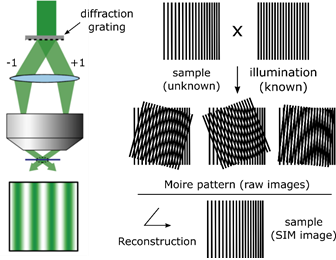
\includegraphics[width=0.91\textwidth]{abbildungen/SIMMMV.png} % Lädt das Bild, skaliert es auf 80% der Textbreite
	\caption{ muss noch was sagen \parencite{OxInstSIMBild}} % Die Bildunterschrift
	\label{fig:SIMBild} % Ein Label für Querverweise (z.B. "siehe Abbildung \ref{fig:beispielbild}")
\end{figure}
Sehr kleine Strukturen weisen hohe räumliche Frequenzen auf. Diese liegen
teilweise außerhalb des Frequenzbereichs, den das Mikroskop aufgrund seiner
begrenzten Auflösung übertragen kann. Durch die Überlagerung der hochfrequenten
Strukturen der Probe mit dem bekannten Beleuchtungsmuster entstehen jedoch
zusätzliche Frequenzanteile. Dabei wird ein Teil der ursprünglich nicht direkt
erfassbaren hochfrequenten Information in einen niedrigeren Frequenzbereich
verschoben, der vom Mikroskop detektiert werden kann. Im aufgenommenen Bild
erscheint diese Wechselwirkung zwischen dem bekannten Beleuchtungsmuster und
den Strukturen der Probe als sogenanntes Moiré-Muster.
Um möglichst viele Informationen über die Probe zu erhalten, wird das
Beleuchtungsmuster in verschiedene Richtungen gedreht und verschoben. Bei der
2D-SIM werden dafür typischerweise neun Einzelaufnahmen und bei der 3D-SIM 15
Einzelaufnahmen aufgenommen. (Haben wir 2 oder 3d gemacht?)
Anschließend werden die Einzelaufnahmen mithilfe von Softwares zu einem Bild
verarbeitet.

Neben der WF Mikroskopie wurde die SIM Mikroskopie eingesetzt, da die höhere
räumliche Auflösung der SIM Mikroskopie für die Fragestellungen der Arbeit von
Bedeutung ist. Die Wide Field Mikroskopie ermöglicht zwar eine Darstellung der
fluoreszenzmarkierten Proteine, weshalb sie sich grundsätzlich zur Untersuchung der
Proben eignet. Jedoch kommt es bei sehr kleinen oder dicht beieinander liegenden

Strukturen dazu, dass sich ihre Fluoreszenzsignale nicht eindeutig voneinander
unterscheiden lassen. Zudem findet bei der WF Mikroskopie keine optische
Schnittbildung statt, da nicht nur eine bestimmte Ebene angeregt wird, sondern auch
Fluorophore anderer Ebenen fluoreszieren. Dies ist bei der Untersuchung der
Kolokalisation zu beachten, da eine scheinbare Überlagerung von Signalen nicht
zwangsläufig einer tatsächlichen räumlichen Übereinstimmung der untersuchten
Strukturen entspricht. Durch den Einsatz der SIM Mikroskopie können die
fluoreszenzmarkierten Strukturen detaillierter dargestellt und die
Kolokalisationsflächen dadurch genauer untersucht werden. Die zusätzliche
Verwendung der Wide Field Mikroskopie ermöglicht einen größeren Überblick mit
schneller Aufnahmegeschwindigkeit über die Zellproben.\footcite{oxinstSIM}
\section{Begründung der Methodenwahl}
können wir glaub weg machen und lieber den einzelnen Methoden Kapitelchen geben evt
\section{Material}
\chapter{Durchführung der praktischen Untersuchungen}
\textbf{Kushagr Sinha}


Der experimentelle Teil lässt sich in zwei Versuche gliedern:

\begin{enumerate}
	\item \textbf{Lokalisation von Caspr2 an Synapsen:} Das Ziel war es,
	die Caspr2-Proteine sowohl an erregenden als auch an
	hemmenden Synapsen zu lokalisieren.
	\item \textbf{Einfluss von Caspr2-Antikörpern auf die
		Protein-Interaktion:} Spezifisch wurde untersucht, ob die
	Interaktion zum Protein Contactin-2 durch Caspr2-AK, gerichtet
	gegen die Discoidin- sowie Laminin1-Domänen, gestört wird.
\end{enumerate}

Um die Experimente beginnen zu können, wurden zunächst
Gehirnzellenkulturen, spezifisch Hippocampus-Neuronkulturen, benötigt. Dafür
werden aus einer trächtigen Maus die Embryonen entnommen, dekapitiert
und die Zellen aus der Hippocampus-Region des Gehirns entnommen.

%Die Zelldichte ist so hoch, dass sie zu Ungenauigkeiten führen würde. Daher wurden die Zellen voneinander getrennt und verdünnt. Dafür werden sie erst enzymatisch mit Trypsin behandelt, welches das Gewebe
%lockert, damit diese beim Triturieren nicht zerquetscht werden.
%Triturieren bezeichnet in diesem Zusammenhang das mechanische Vereinzeln
%von Zellen durch Auf- und Abpipettieren der Gewebestücke.

Um die Zellen aus dem dichten Gewebe voneinander zu trennen und zu vereinzeln, werden sie zuerst mit dem Enzym Trypsin behandelt. Trypsin spaltet die Peptidverbindungen zwischen den Zellen und lockert somit das Gewebe auf. Nach ca. fünf Minuten wird das Gewebe mit einem Medium (HBSS) gewaschen, das heißt, Lösung hinzugeben, kurz warten und schließlich abpipettieren, um das Enzym zu entfernen und die Enzymreaktion zu stoppen. Dadurch werden die Zellen beim anschließenden Triturieren (dem mechanischen Vereinzeln durch Auf- und Abpipettieren der Gewebestücke) nicht beschädigt.
%Danach werden diese mit einer Zellsuspensionslösung versetzt und auf die
%gewünschte Zelldichte verdünnt (ca.\ 20.000~Zellen/cm$^2$). Jetzt
%werden die Zellen auf Deckgläschen verteilt, welche vorher mit
%Poly-D-Lysin beschichtet wurden, um eine haftende Oberfläche für die
%Zellen zu schaffen. Damit die Zellen dann auch ein neuronales Netzwerk
%ausbilden, werden diese mit einem Neurobasal-Medium (NB), welches
%Nährstoffe und Wachstumsfaktoren enthält, versetzt und anschließend 14~Tage
%inkubiert.

Durch diesen Vorgang entsteht eine Zellsuspension, wobei die Zellen einzeln in dem Medium herumschweben (= Suspension). Mithilfe einer Zählkammer und verschiedener Berechnungen wird diese mit einem Medium verdünnt, um somit die gewünschte Zelldichte zu erreichen (ca.\ 20.000 Zellen/cm$^2$). Im Anschluss werden die Zellen auf Deckgläschen verteilt, welche vorher mit Poly-D-Lysin beschichtet wurden, um eine haftende Oberfläche für die Zellen zu schaffen. Damit die Zellen dann auch ein neuronales Netzwerk ausbilden, werden diese mit einem Neurobasal-Medium (NB), welches Nährstoffe und Wachstumsfaktoren enthält, versetzt und anschließend 14 Tage im Brutschrank bei 37 °C inkubiert. 

%Danach wurden die Zellen kurz vor dem Anfang der Färbungen 20 Minuten lang mit einer 4\%igen PFA-Lösung behandelt und damit fixiert. Fixieren bedeutet, die Proteine chemisch zu stabilisieren und die Zelle in ihrem aktuellen Zustand \glqq einzufrieren\grqq{}; allerdings stirbt die Zelle dabei.
% ────────────────────────────────────────────────────────────
\section{Untersuchung zur Lokalisation von Caspr2 an Synapsen}
% ────────────────────────────────────────────────────────────

%Der gesamte Prozess zur Immunfärbung der Zellkulturen dauerte drei Tage.
%Insgesamt wurden elf Deckgläschen verwendet (siehe Tabelle~\ref{tab:proben}), welche
%in verschiedene Versuchsgruppen unterteilt wurden. Am ersten Tag
%wurden die Zellen nach dem Fixieren dreimal gewaschen, das heißt Lösung hinzugeben, kurz warten und dann abpipettieren (siehe Abbildung \ref{fig:waschV}). Dies wurde immer mit PBS (Phosphat-gepufferte Salzlösung) gemacht. Das PBS wurde benutzt, da es eine isotonische, nicht-toxische Lösung ist,
%die den pH-Wert stabilisiert und die Zellen schont.


Der gesamte Prozess zur Immunfärbung der Zellkulturen dauerte drei Tage.
Insgesamt wurden elf Deckgläschen verwendet (siehe Tabelle~\ref{tab:proben}), welche
in verschiedene Versuchsgruppen unterteilt wurden. 

Am ersten Tag wurden die Zellen kurz vor dem Anfang der Färbungen 20 Minuten lang mit einer 4\%igen PFA-Lösung behandelt und damit fixiert. Fixieren bedeutet, die Proteine chemisch zu stabilisieren und die Zelle in ihrem aktuellen Zustand \glqq einzufrieren\grqq{}; allerdings stirbt die Zelle dabei. Darauffolgend wurden sie dreimal mit PBS (Phosphat-gepufferte Salzlösung) gewaschen (siehe Abbildung \ref{fig:waschV}). Das PBS wurde benutzt, da es eine isotonische, nicht-toxische Lösung ist, die den pH-Wert stabilisiert und die Zellen schont.

Nachdem die Zellen dreimal gewaschen wurden, wurde ein Puffer~B1
aufgetragen, welcher aus 10\%iger BSA-Lösung (Rinderserumalbumin) und
10\%iger NDS-Lösung (normales Eselserum) bestand und als
Blockierungslösung diente. Dabei dient der Puffer dazu, unspezifische
Bindungsstellen auf den Deckgläschen und auf den Zellen zu besetzen. Dies
stellt sicher, dass die später hinzugefügten AK nur an ihre spezifischen
Zielproteine binden und keine störende Hintergrund-Fluoreszenz verursachen.

Nach einer Stunde Einwirkzeit wurde der Puffer~B1 abpipettiert und die
ersten Primärantikörper (Caspr2 bzw.\ der Kontrollantikörper)
hinzugefügt. Diese wurden anschließend über Nacht bei 4\,°C
inkubiert.

% ── Bild 1 ausgelassen ───────────────────────────────────────
\clearpage
\begin{table}[htbp]
	\centering
	\caption{Übersicht der elf Proben des ersten Versuches.}
	\label{tab:proben}
	\setlength{\tabcolsep}{3pt} % Verringert den seitlichen Abstand in den Zellen
	\begin{tabularx}{\textwidth}{c >{\raggedright\arraybackslash}X c >{\raggedright\arraybackslash}X c >{\raggedright\arraybackslash}X}
		\toprule
		\textbf{Nr.} & \textbf{Färbung} &
		\textbf{Nr.} & \textbf{Färbung} &
		\textbf{Nr.} & \textbf{Färbung} \\
		\midrule
		(1) & Caspr2 + VGlut1 &
		(5) & Caspr2 + VGat &
		(9) & Kontrolle + VGlut1 \\
		(2) & Caspr2 + VGlut1 &
		(6) & Caspr2 + VGat &
		(10) & Kontrolle + VGat \\
		(3) & Caspr2 + VGlut1 &
		(7) & Caspr2 + VGat &
		(11) & Negativkontrolle (nur SEK1+2) \\
		(4) & Caspr2 + VGlut1 &
		(8) & Caspr2 + VGat &
		& \\
		\bottomrule
	\end{tabularx}
\end{table}

\begin{figure}[h]
	\centering
	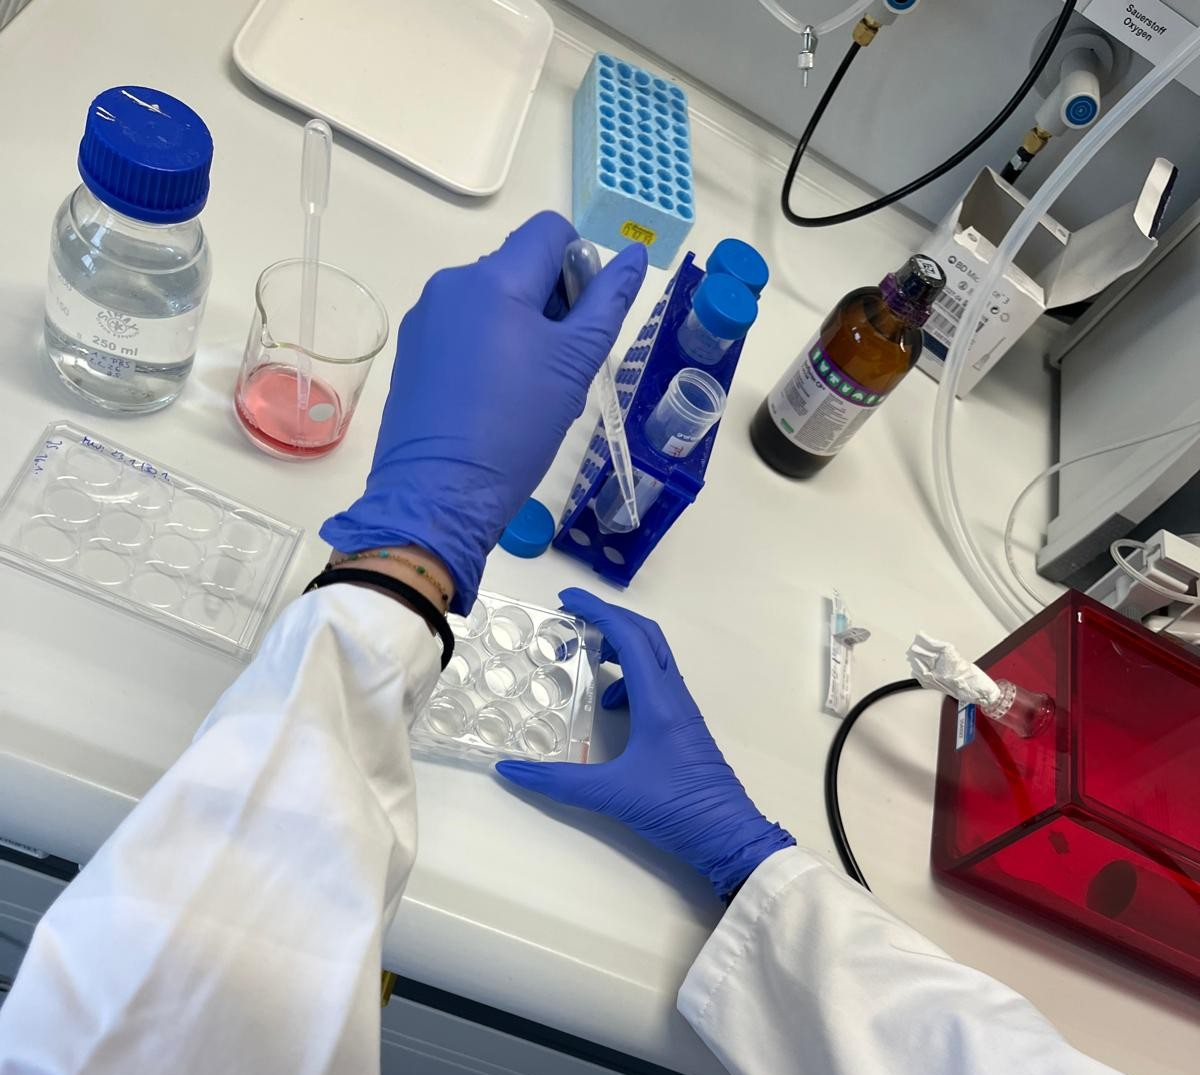
\includegraphics[width=0.75\textwidth]{abbildungen/waschvorgangDPU.jpeg}
	\caption{Vorgang des Fixierens und Waschens \parencite{eigenAu6.1}}
	\label{fig:waschV}
\end{figure}
Am zweiten Tag wurden die Deckgläschen in eine Feuchtekammer
transferiert. Dies ist notwendig, damit die geringen Mengen an
Antikörperlösung während der Einwirkzeit nicht verdunsten und die Zellen nicht austrocknen. Die Kammer
bestand aus einer Plastikbox mit angefeuchteten Papiertüchern als
Untergrund (siehe Abbildung \ref{fig:fKammer}).
\clearpage
% (siehe Bild 2)
\begin{figure}[h]
	\centering
	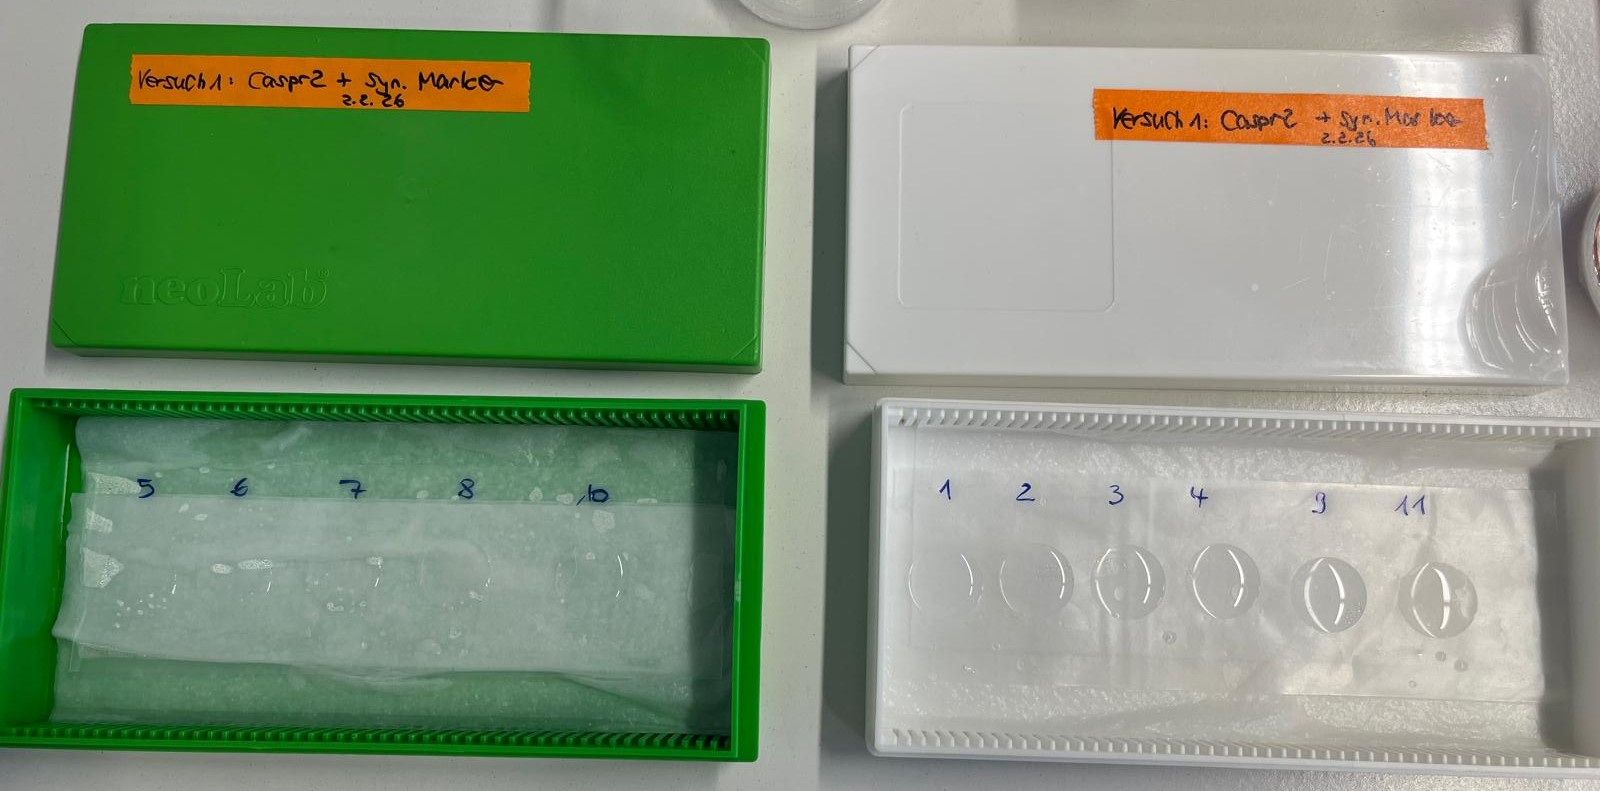
\includegraphics[width=1\textwidth]{abbildungen/fkammerDPU.jpeg}
	\caption{Feuchtekammer \parencite{eigenAu6.2}}
	\label{fig:fKammer}
\end{figure}

Nach sechsmaligem Waschen mit PBS wurden die ersten Sekundärantikörper, nämlich AF647@sheep, hinzugegeben. Die Bezeichnung \glqq AF647\grqq{} gibt dabei an, dass der Antikörper mit dem Fluoreszenzfarbstoff AF647 markiert ist, der bei einer Wellenlänge von 647 nm emittiert. \glqq Sheep\grqq{} bezeichnet hingegen die Spezies, gegen die die Sekundärantikörper gerichtet sind. Da der erste Primärantikörper gegen Caspr2 gerichtet ist und aus dem Schaf stammt, bindet der gegen Schaf gerichtete Sekundärantikörper an diesen Primärantikörper. Nach einer Inkubationszeit von zwei Stunden wurde die Deckgläschen erneut sechsmal mit PBS gewaschen.

%Um die Zellen für die zweiten Primärantikörper besser zugänglich zu
%machen, wurde eine Pufferlösung~B2 hergestellt. Diese bestand aus der
%B1-Lösung und zusätzlich Triton. Das Triton dient dazu, kleine Löcher
%in die Zellmembran zu machen, damit die VGlut/VGat-Antikörper auch in
%das Innere der Synapse gelangen und binden können. Diese wurden nach der
%Puffer-Behandlung hinzugefügt und erneut über Nacht bei 4\,°C gelagert.

Wichtige Proteine von Synapsen sind VGlut und VGat. Da sich diese allerdings nicht auf der Membranoberfläche, sondern im Inneren der Zelle befinden, muss erst ein Zugang durch die fixierte Zellmembran geschaffen werden, damit die Antikörper daran binden können.

Um die Zellen für diese Antikörper zugänglich zu machen, wurde die Pufferlösung B2 hergestellt. Diese bestand aus der B1-Lösung und zusätzlich dem Detergenz Triton. Triton wirkt ähnlich wie Seife und kann Fette lösen. Da die Zellmembran aus Fettsäuren besteht, \glqq wäscht\grqq{} das Triton kleine Löcher in die Membran. So können die VGlut- und VGat-Antikörper, die in Meerschweinchen gezüchtet wurden, in das Innere der Synapse gelangen und binden. Die Zugabe erfolgte nach der Puffer-Behandlung mit anschließender Inkubation über Nacht bei 4\,°C.

Am dritten Tag wurde die Lösung wieder sechsmal mit PBS abgewaschen, und
es folgte die Zugabe der zweiten Sekundärantikörper, CF488@gp (fluoresziert
grün und ist gerichtet gegen Meerschweinchen-AK), gegen VGlut- und
VGat-AK. Nach zwei Stunden wurde sechsmal abgewaschen.

Anschließend wurde DAPI hinzugefügt, eine Lösung, die den Zellkern
anfärbt, indem sie mit der darin vorhandenen DNA interagiert. Damit wurde erzielt, dass die Zellen unter dem Mikroskop einfacher zu finden sind.

Diese wurden dann dreimal gewaschen. Zehn Minuten lang wurden die
Präparate dann nochmals mit einer 4\%igen PFA-Lösung fixiert, damit sie über Monate hinweg
mikroskopiert werden können. Nach einem letzten Waschschritt waren die
Präparate fertig für die Auswertung.

\section{Untersuchung zum Einfluss von humanen Caspr2-Antikörpern auf die Protein-Interaktion mit Contactin-2}

Im zweiten Versuchsteil wurde untersucht, ob die Bindung von humanen Caspr2-Antikörpern (aus Patientenseren) die Interaktion zwischen Caspr2 und dem Bindungspartner Contactin-2 beeinträchtigt oder blockiert.
Der Ablauf gliederte sich erneut in drei Tage mit mehreren Aufbereitungsschritten.

%

%Der erste Tag der Färbungen fing damit an dass die noch lebenden Zellen mit den zuvor erwähnten humanen AK behandelt wurden. DAbei gab es 2 verschieden ARten, eine die daen Laminin1 Domänene angegriffen ahben und die anderen die den Discoidin Domäne angegriffen haebn. Damit entstanden insgesamt 12 PRoben wie in Tabelle \ref{tab:proben2} zu sehen sind.

%Zu Beginn wurden die benötigten Neurobasal-Medien vorbereitet und auf 37 °C erwärmt. Für die Behandlung der Neuronenkulturen wurden drei verschiedene Ansätze hergestellt. Für die Discoidin gerichteten AK wurden 20 µl Discoidin mit 2600 µl Neurobasal-Medium versetzt. Für die Laminin-Bedingung wurden 17,93 µl Laminin mit 2600 µl Neurobasal-Medium gemischt. Als Kontrolle wurden 10,83 µl MGO-53 mit 1300 µl Neurobasal-Medium angesetzt. Anschließend wurden die entsprechenden Ansätze zu den Neuronenkulturen gegeben. Die Kulturen wurden für 24 Stunden bei 37 °C inkubiert.


Zu Beginn des ersten Tages des Versuches wurde zur Vorbereitung Neurobasal-Medium auf 37 \,°C erwärmt. Damit konnten die verschiedenen benötigten Ansätze mit humanen monoklonalen Caspr2-Antikörpern gegen Discoidin oder Laminin-1 hergestellt werden. Außerdem gab es noch einen Kontroll-Antikörper, mgo-53, mit demselben Ziel wie im ersten Versuch genannt.

 Als diese Primär-Antikörper mit dem Neurobasal-Medium auf die benötigte Konzentration verdünnt wurden, wurden jeweils 500 µl in jedes Well getropft. Anschließend wurden sie bei 37 \,°C 24 Stunden lang inkubiert. Damit entstanden insgesamt 12 Proben, wie in Tabelle \ref{tab:proben2} zu sehen ist.

\begin{table}[htbp]
	\centering
	\caption{Übersicht der zwölf Proben des zweiten Versuches.}
	\label{tab:proben2}
	\setlength{\tabcolsep}{3pt} % Verringert den seitlichen Abstand in den Zellen
	\begin{tabularx}{\textwidth}{c >{\raggedright\arraybackslash}X c >{\raggedright\arraybackslash}X c >{\raggedright\arraybackslash}X}
		\toprule
		\textbf{Nr.} & \textbf{Färbung} &
		\textbf{Nr.} & \textbf{Färbung} &
		\textbf{Nr.} & \textbf{Färbung} \\
		\midrule
		(1) & Discoidin + Contactin-2 &
		(5) & Laminin1 + Contactin-2 &
		(9) & Control + Contactin-2 \\
		(2) & Discoidin + Contactin-2 &
		(6) & Laminin1 + Contactin-2 &
		(10) & Control + Contactin-2 \\
		(3) & Discoidin + Contactin-2 &
		(7) & Laminin1 + Contactin-2 &
		(11) & negative control (nur SEK1+2) \\
		(4) & Discoidin + Contactin-2 &
		(8) & Laminin1 + Contactin-2 &
		(12) & negative control (nur SEK1+2) \\
		\bottomrule
	\end{tabularx}
\end{table}
Am zweiten Tag der Färbung wurden die Neuronen auf den Deckgläschen zunächst dreimal kurz bei 37\,°C mit erwärmtem Neurobasal-Medium gewaschen. Anschließend wurden die Zellen für 20~Minuten bei Raumtemperatur mit einer 4\,\%igen PFA-Lösung behandelt, um sie in ihrem aktuellen Zustand zu fixieren und chemisch zu stabilisieren. Nach der Fixierung folgte ein dreimaliger Waschschritt mit PBS für jeweils 5~Minuten, um Reste des Fixiermittels gründlich zu entfernen.

Zur Vermeidung unspezifischer Antikörperbindungen wurden die Präparate danach für eine Stunde bei Raumtemperatur mit dem Puffer B1 inkubiert. Dieser bestand aus einer Mischung aus 10\,\%iger BSA-Lösung und 10\,\%igem NGS (normales Ziegenserum / Normal Goat Serum) in PBS. Das NGS blockiert, genau wie das NDS im vorherigen Versuch, die freien Bindungsstellen auf der Oberfläche.




Da die Zellen bereits mit humanen Caspr2-Antikörpern behandelt worden waren, folgte im nächsten Schritt direkt die Zugabe des ersten Sekundärantikörpers. Hierfür wurde der Puffer SEK1, bestehend aus 1\,\% BSA, 1\,\% NGS und dem Antikörper CF640R@hu, aufgetragen und für 2~Stunden bei Raumtemperatur inkubiert. Der Antikörper CF640R@hu ist spezifisch gegen humane Antikörper gerichtet und trägt den Fluoreszenzfarbstoff CF640R (Emissionswellenlänge im fernroten Bereich bei ca.~640\,nm), wodurch die gebundenen Caspr2-Antikörper sichtbar gemacht werden.

Nach Ablauf der Inkubationszeit wurden die Deckgläschen sechsmal für jeweils 5~Minuten mit PBS gewaschen. Danach wurde der Puffer PRIM2 aufgetragen, welcher den gegen Contactin-2 gerichteten Primärantikörper (in Kaninchen gezüchtet) sowie 1\,\% BSA und 1\,\% NGS enthielt. Die Inkubation erfolgte über Nacht bei 4\,°C in der Feuchtekammer.

Am darauffolgenden Tag wurden die Proben erneut sechsmal für jeweils 5~Minuten mit PBS gewaschen, um ungebundene Contactin-2-Antikörper zu entfernen. Im Anschluss wurde der zweite Sekundärantikörper über den Puffer SEK2 (1\,\% BSA, 1\,\% NGS und CF568@rb) hinzugegeben. Dieser Antikörper bindet spezifisch an Kaninchen-Antikörper und fluoresziert durch den Farbstoff CF568 in roter Farbe. Die Inkubationszeit betrug zwei Stunden bei Raumtemperatur.

Nach erneutem sechsmaligem Waschen mit PBS wurde für 5~Minuten DAPI hinzugefügt. DAPI diente wieder als Orientierungshilfe bei der Mikroskopie. Nach drei kurzen Waschschritten mit PBS wurden die Präparate nochmals für 10~Minuten bei Raumtemperatur mit einer 4\,\%igen PFA-Lösung nachfixiert, um die gebildeten Antikörper-Protein-Komplexe dauerhaft zu stabilisieren.
\clearpage
Nach drei finalen kurzen Waschschritten mit PBS wurden die Deckgläschen, aus dem ersten Versuch sowie dem zweiten Versuch, schließlich mit dem Eindeckmedium Fluoromount auf Objektträgern eingedeckt (siehe Abbildung \ref{fig:objtr}). Fluoromount schützt das Präparat vor dem Austrocknen und verhindert das Ausbleichen der Fluoreszenzfarbstoffe, sodass die Proben mithilfe des SIM-Mikroskops ausgewertet werden können.
\begin{figure}[h]
	\centering
	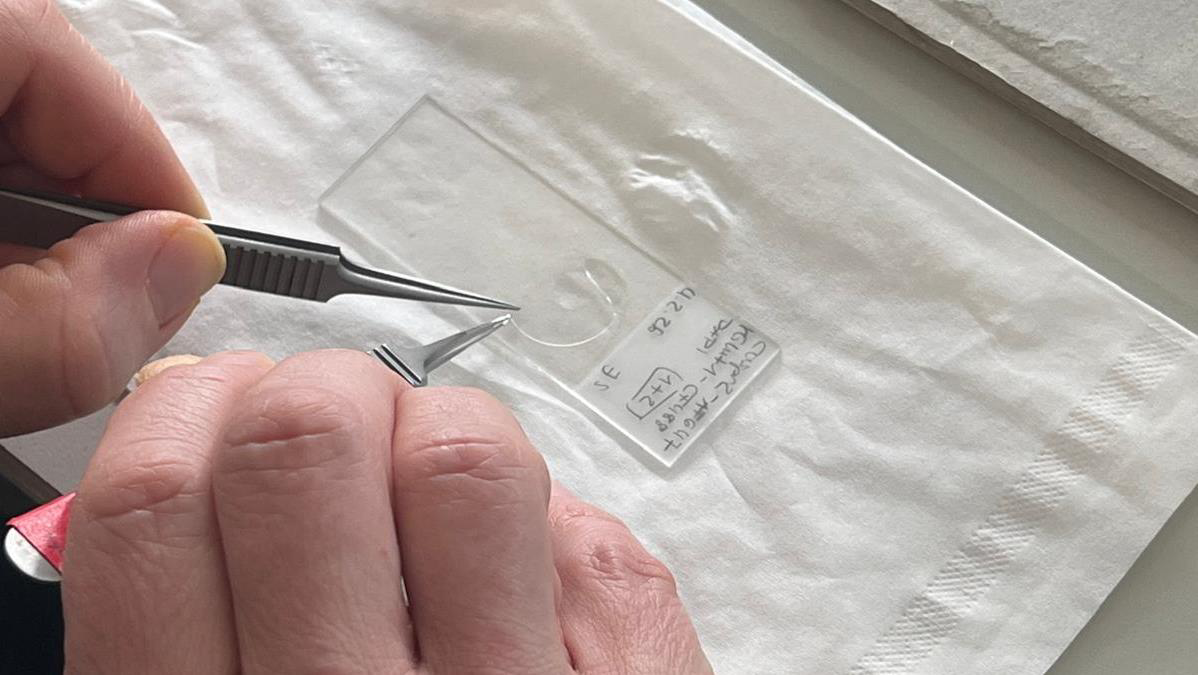
\includegraphics[width=1\textwidth]{abbildungen/objektträgerDPU.png}
	\caption{Feuchtekammer \parencite{eigenAu6.3}}
	\label{fig:objtr}
\end{figure}


\chapter{Ergebnisse und Auswertung}
\textbf{Helene Becker}
%    \section{Auswertung der Ergebnisse}
%    \section{Darlegung der Ergebnisse}
\section{Kolokalisation von Caspr2 mit VGat und VGlut}

Zur Untersuchung der synaptischen Lokalisation von Caspr2 wurden die
synaptischen Marker VGat und VGlut angefärbt. VGat dient als Marker für
inhibitorische Synapsen und VGlut als Marker für exzitatorische Synapsen.
Anhand Structured Illumination Microscopy (SIM) und Wide Field (WF)
wurden die Färbungen analysiert und die Kolokalisation wurde als überlappende Fläche von Caspr2 und dem jeweiligen synaptischen Marker in $\mu\text{m}^2$ bestimmt. Die Daten wurden mittels Shapiro-Wilk-Test auf Normalverteilung geprüft. Die Normlverteilung ist die symmmetrische Verteilung der Werte in glockenform. Diese Normalverteilung lag nicht vor, weshalb anschließend der nichtparametrische Mann-Whitney U-Test verwendet wurde. Also ein Test, der nicht an eine bestimmte Verteilung von Daten, wie zum Beispiel die Normalverteilung, gebunden ist.

Die SIM-Daten in Abbildung \ref{fig:coflma} zeigen bei beiden Markern eine geringe Anzahl und
Größe der Kolokalisationsflächen. Der Medianwert bei VGat und VGlut liegt
jeweils bei etwa $1\,\mu\text{m}^2$. Die mittleren 50\,\% der VGat-Werte
liegen im Bereich von ca.\ $0{,}5$--$2\,\mu\text{m}^2$, die VGlut-Analyse
ergab lediglich einen Wert. Die Streuung der SIM-Daten ist gering.

Die WF-Daten weisen eine größere Streuung auf. Hier liegt der Median der VGat-Daten bei rund $1{,}81\,\mu\text{m}^2$ und der der VGlut-Daten bei rund $1{,}32\,\mu\text{m}^2$. Zudem treten zahlreiche Extrema auf. Sie
erreichen Werte von über $10\,\mu\text{m}^2$, teils liegen sie im Bereich
von ca.\ $40$--$95\,\mu\text{m}^2$.

Die ist auf den Unterschied der Verfahren bzgl. der Auflösung zurückzuführen. WF dient häufig dem Aufnehmen von Übersichtsbildern von Strukturen und weißt eine geringere Auflösung auf (siehe Abbildung \ref{fig:WFnerv}). SIM (siehe Abbildung \ref{fig:SIMnerv}) besitzt aufgrund der strukturierten Beleuchtung eine höhere Auflösung. Daher ist für die Auswertung der Versuchsergebnisse im Folgenden die SIM-Methode von Bedeutung. Durch die höhere Auflösung liefert diese eine bessere Trennung von überlagerten Signalen und kann daher als genauer und relevanter für die Ergebnisauswertung angesehen werden. 

In beiden Gruppen liegen die meisten Werte im niedrigen Bereich,
gleichzeitig kommt es zum Auftreten einzelner hoher Werte. Der
statistische Vergleich mittels Mann-Whitney U-Test zeigt
im SIM-Datensatz keinen signifikanten Unterschied zwischen VGat und VGlut
($p = 0{,}257$, n.\,s.).

Mittels Mann-Whitney U-Test konnte kein Nachweis für ein bevorzugtes Vorhandensein von Caspr2 an einem der untersuchten Synapsentypen erbracht werden. Ein möglicher Unterschied ist jedoch nicht auszuschließen.

% ── Abbildung 1 (Boxplot) ausgelassen ───────────────────────
% Abb. 1: Colokalisationsfläche von Caspr2 mit synaptischen
%         Markern VGlut und VGat (SIM und WF)
% ─────────────────────────────────────────────────────────────
\begin{figure}[h] % [h] versucht, das Bild hier zu platzieren (hier), [t] für oben, [b] für unten
	\centering % Zentriert das Bild horizontal
	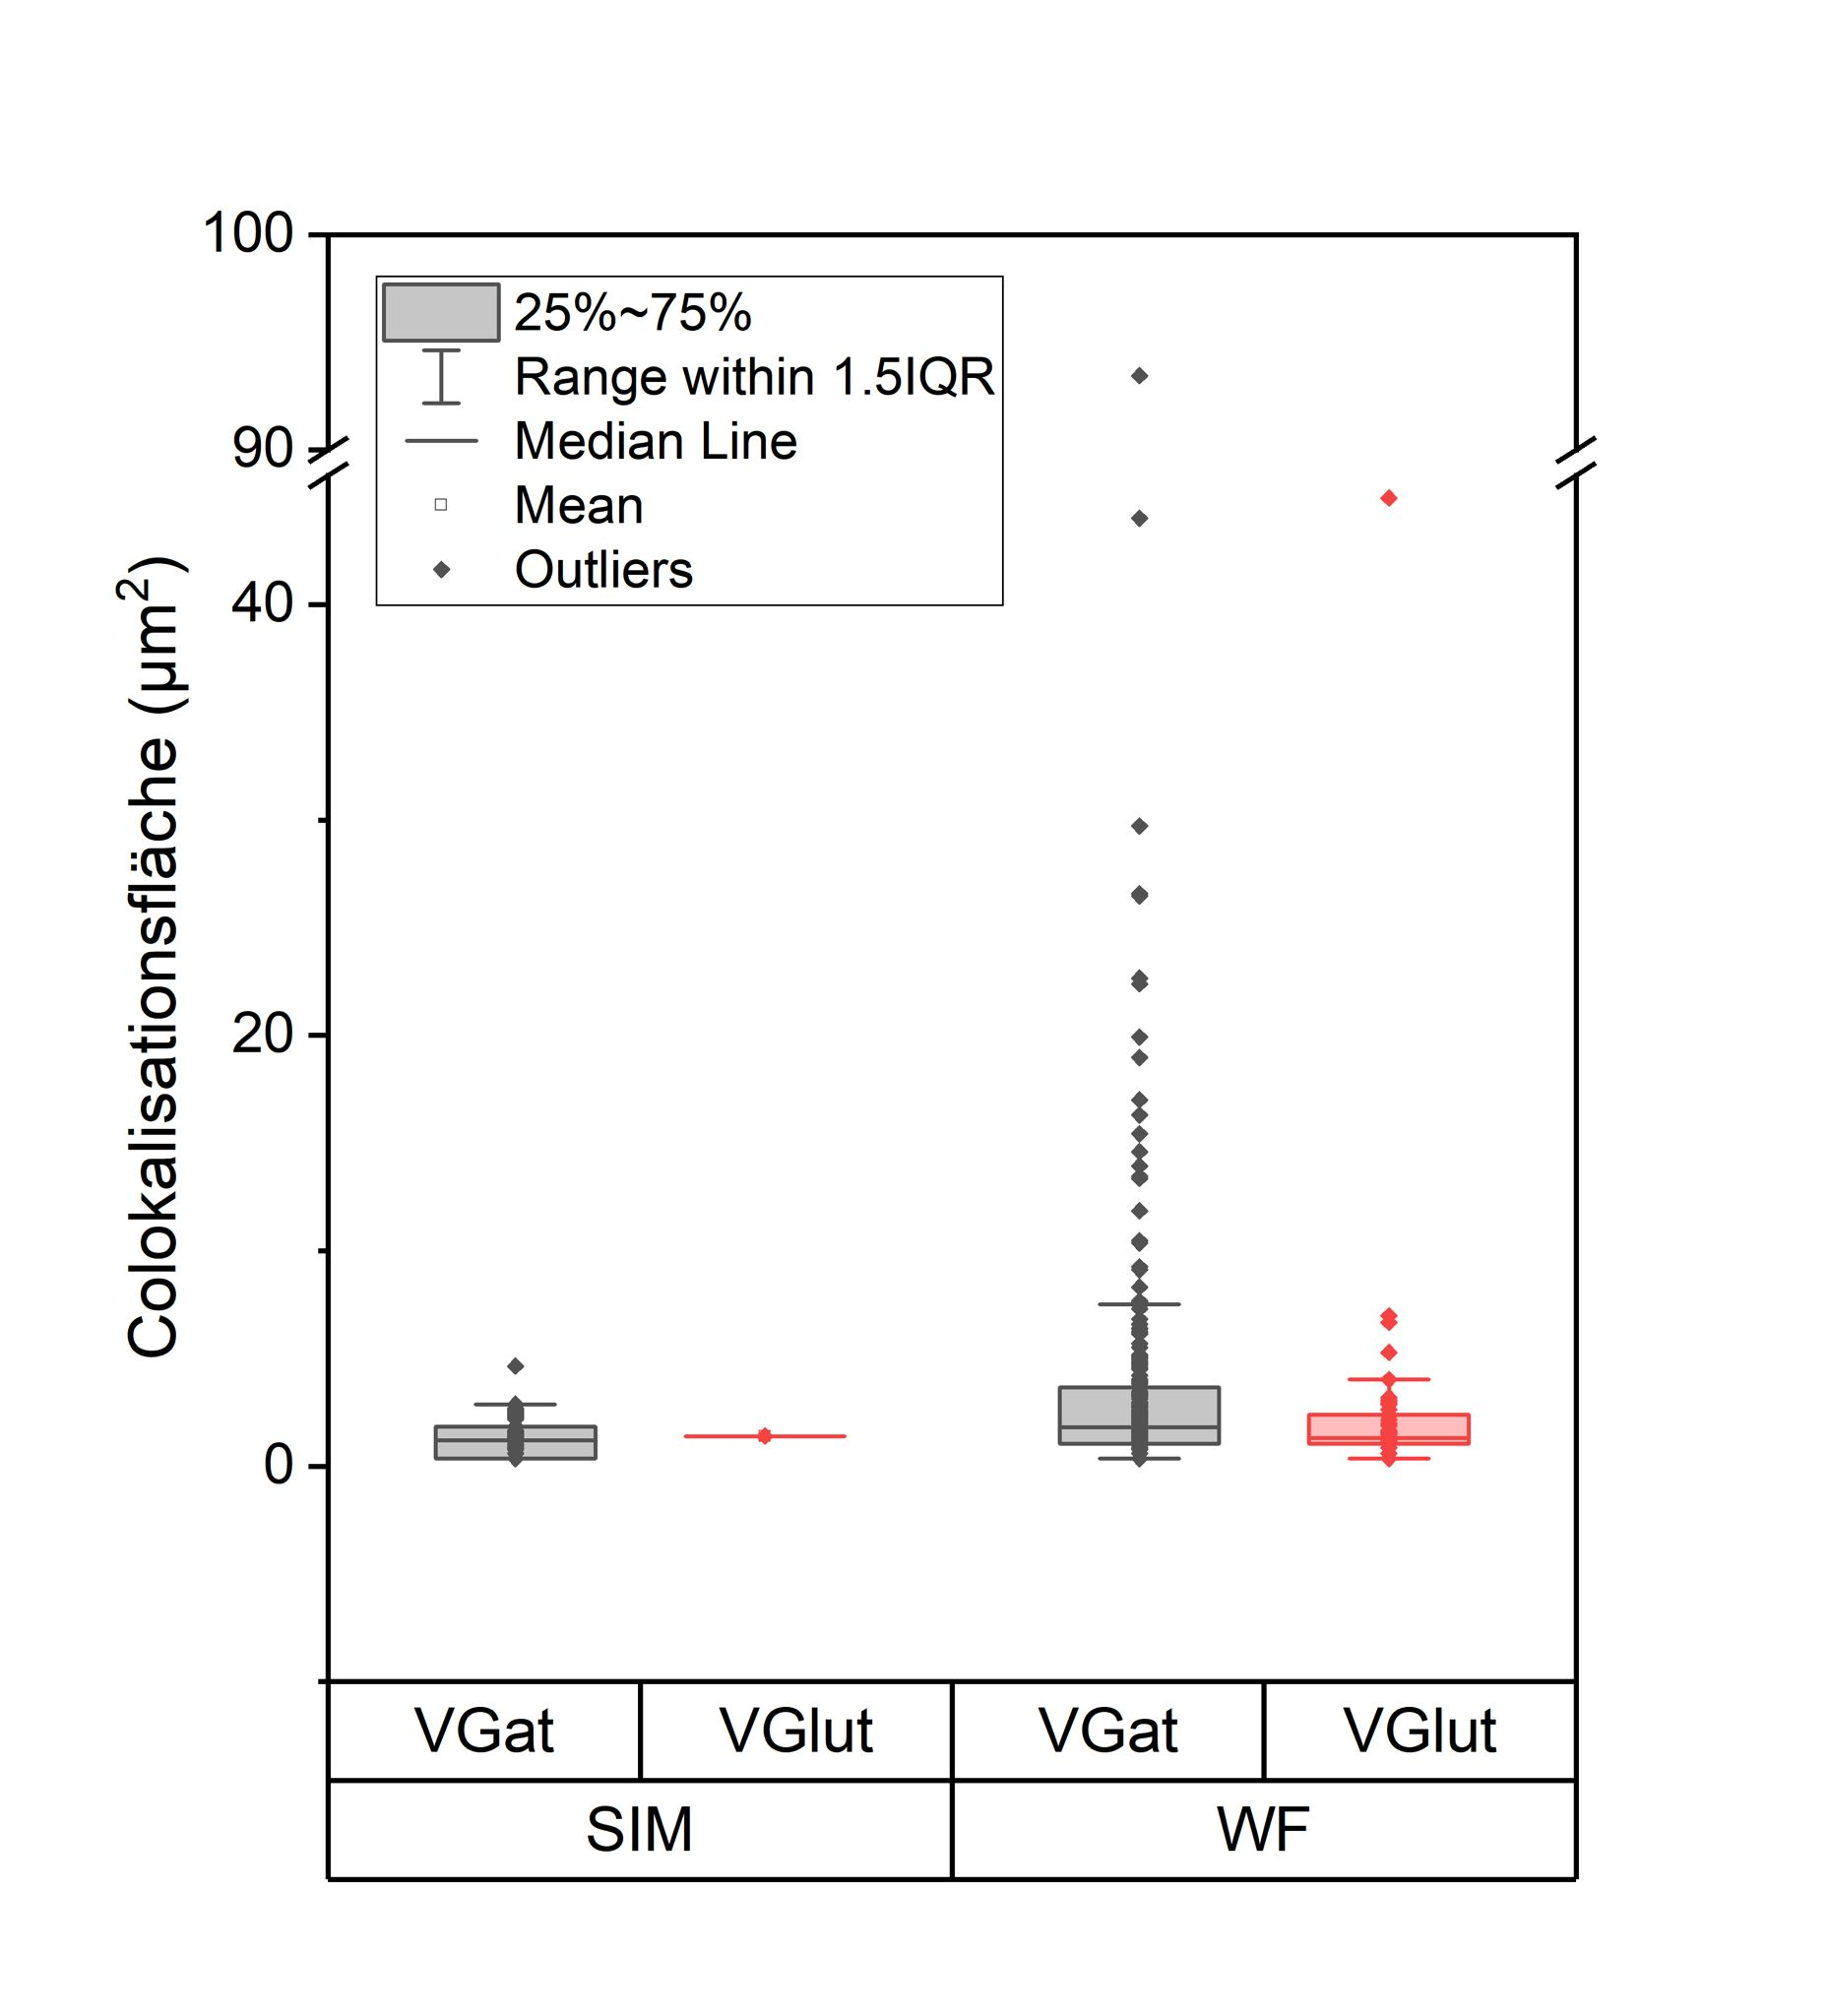
\includegraphics[width=0.8\textwidth]{abbildungen/colokflächemarkerKCVV.jpg} % Lädt das Bild, skaliert es auf 80% der Textbreite
	\caption{Colokalisationsfläche von Caspr2 mit synaptischen
		Markern VGlut und VGat \parencite{eigenAu7.1}} % Die Bildunterschrift
	\label{fig:coflma} % Ein Label für Querverweise (z.B. "siehe Abbildung \ref{fig:beispielbild}")
\end{figure}
\begin{figure}[h] % [h] versucht, das Bild hier zu platzieren (hier), [t] für oben, [b] für unten
	\centering % Zentriert das Bild horizontal
	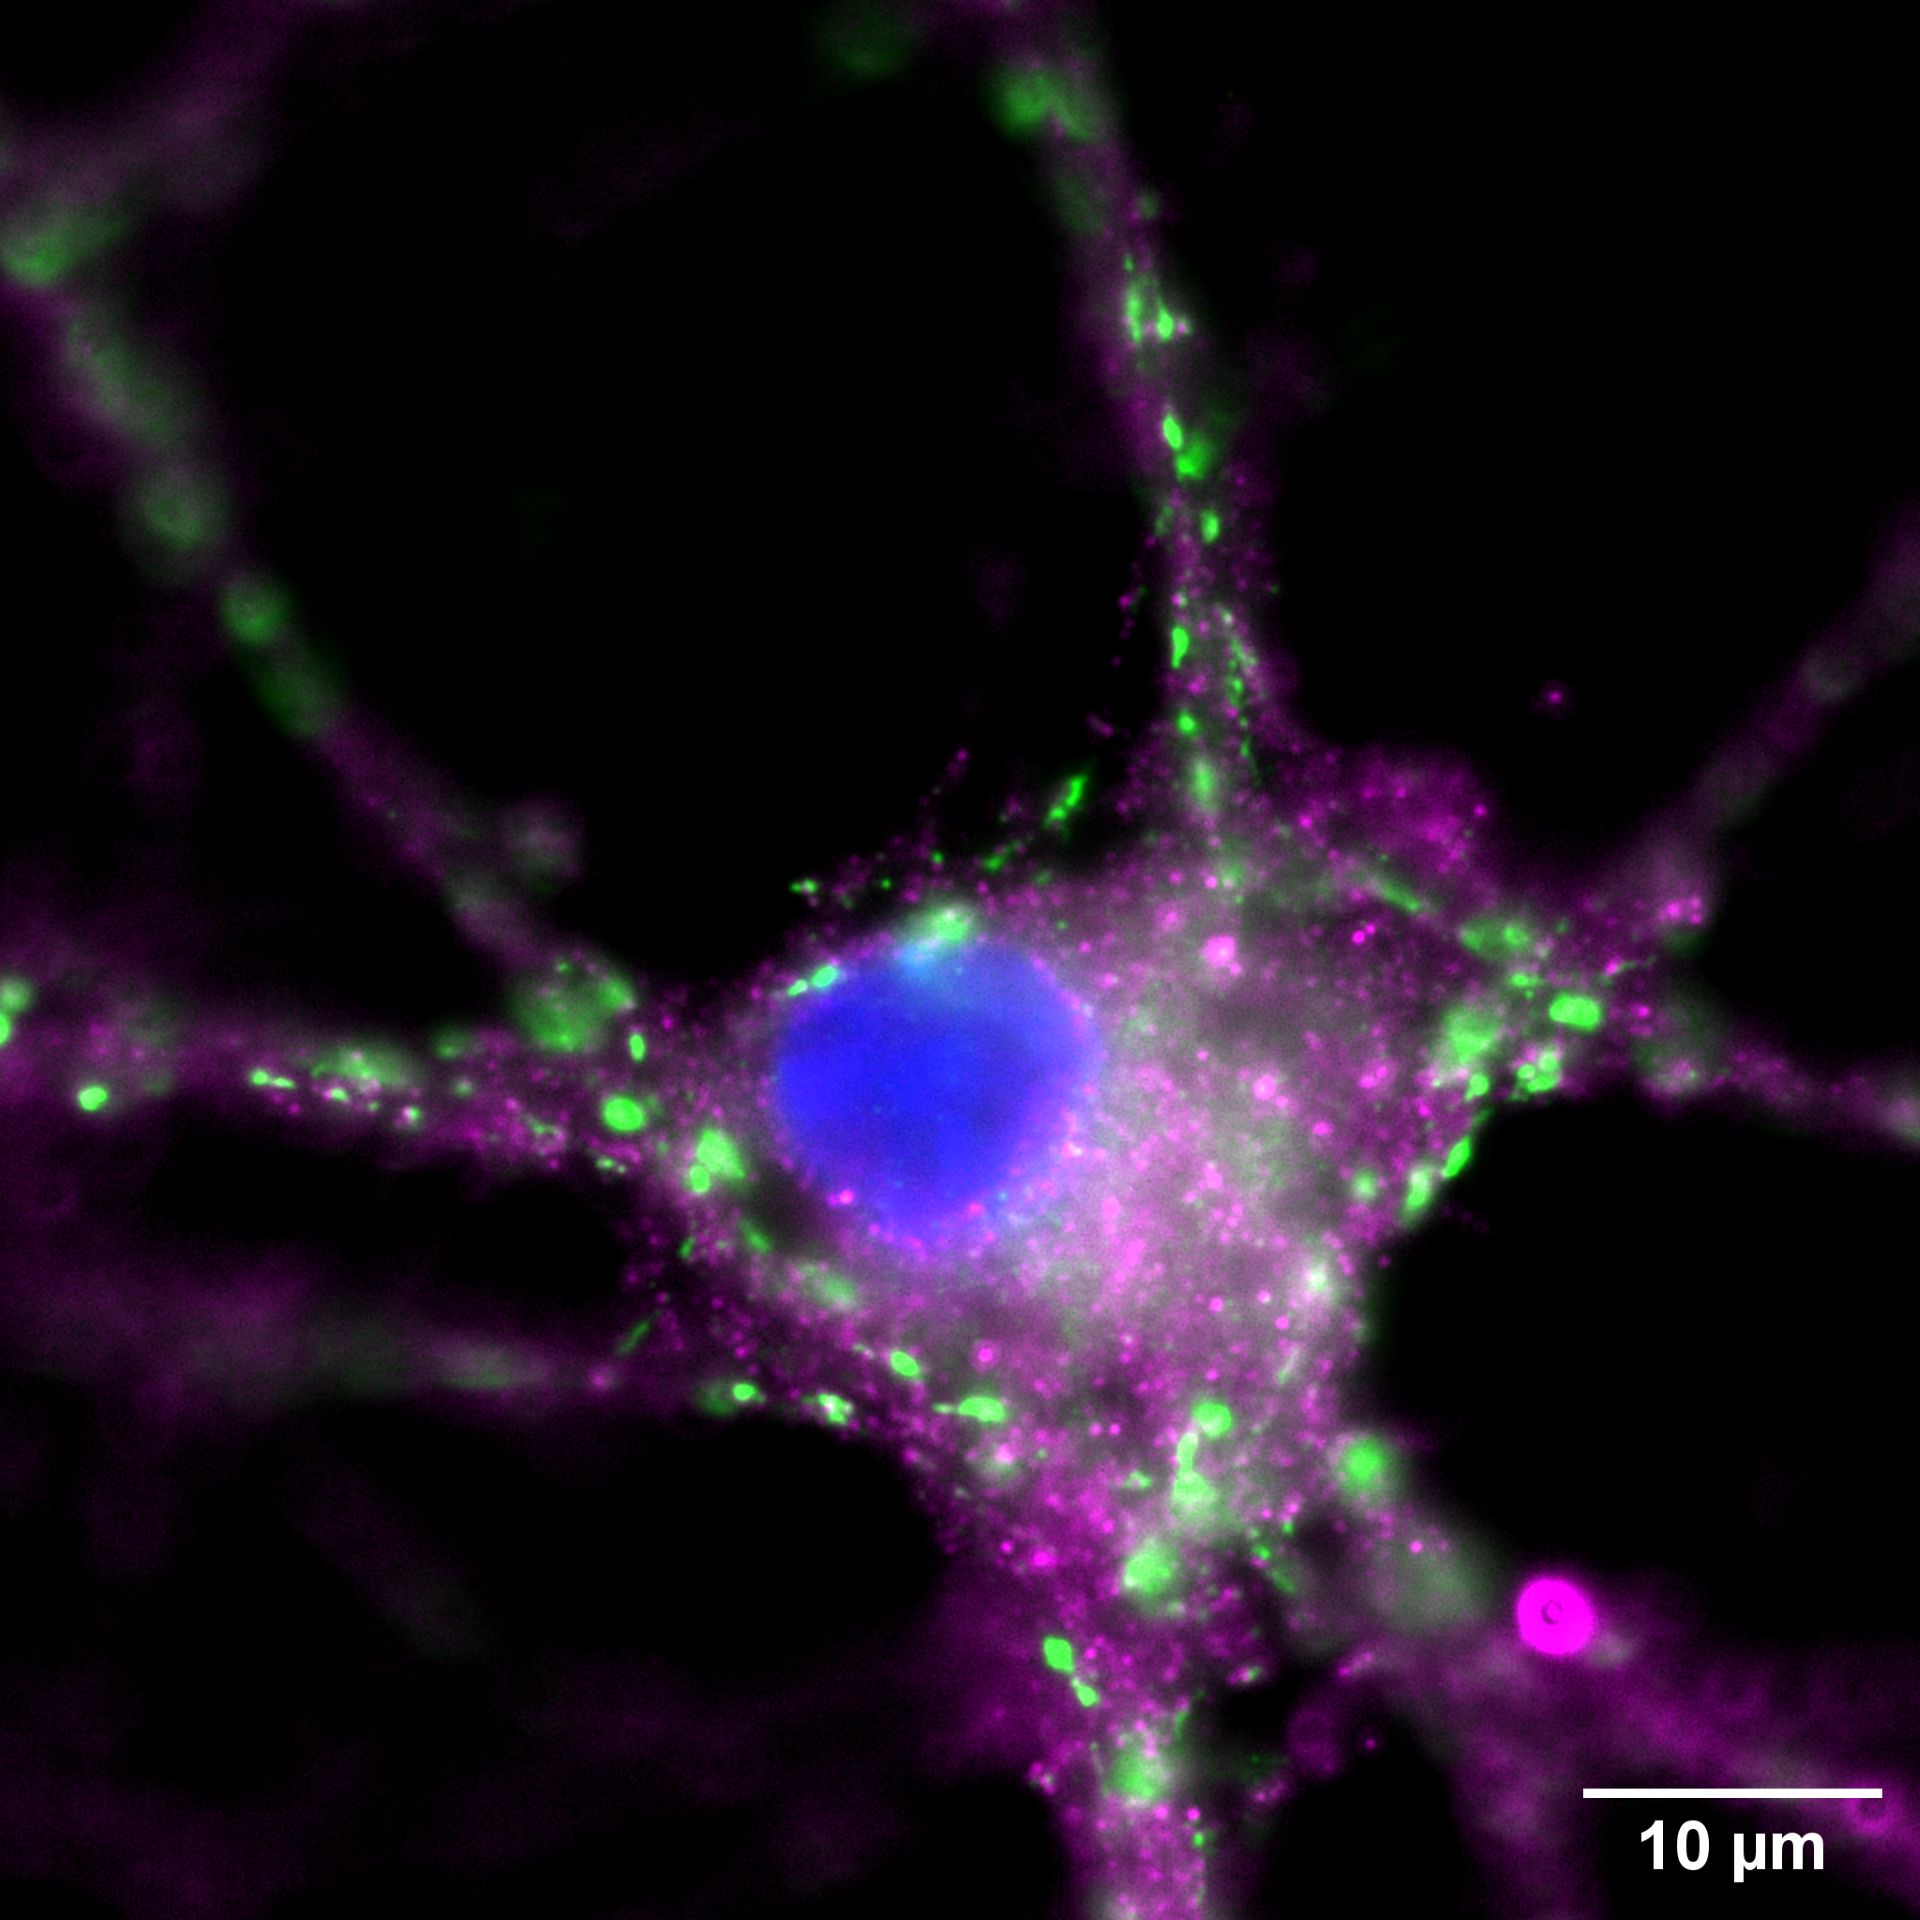
\includegraphics[width=0.8\textwidth]{abbildungen/WFNervEuA.png} % Lädt das Bild, skaliert es auf 80% der Textbreite
	\caption{Wide-Field-(WF)-Aufnahme einer Nervenzelle. Die fluoreszierenden Strukturen zeigen Caspr2 (magenta), VGat (grün) und einen Zellkern (blau) \parencite{eigenAu7.2}} % Die Bildunterschrift
	\label{fig:WFnerv} % Ein Label für Querverweise (z.B. "siehe Abbildung \ref{fig:beispielbild}")
\end{figure}
\begin{figure}[h] % [h] versucht, das Bild hier zu platzieren (hier), [t] für oben, [b] für unten
	\centering % Zentriert das Bild horizontal
	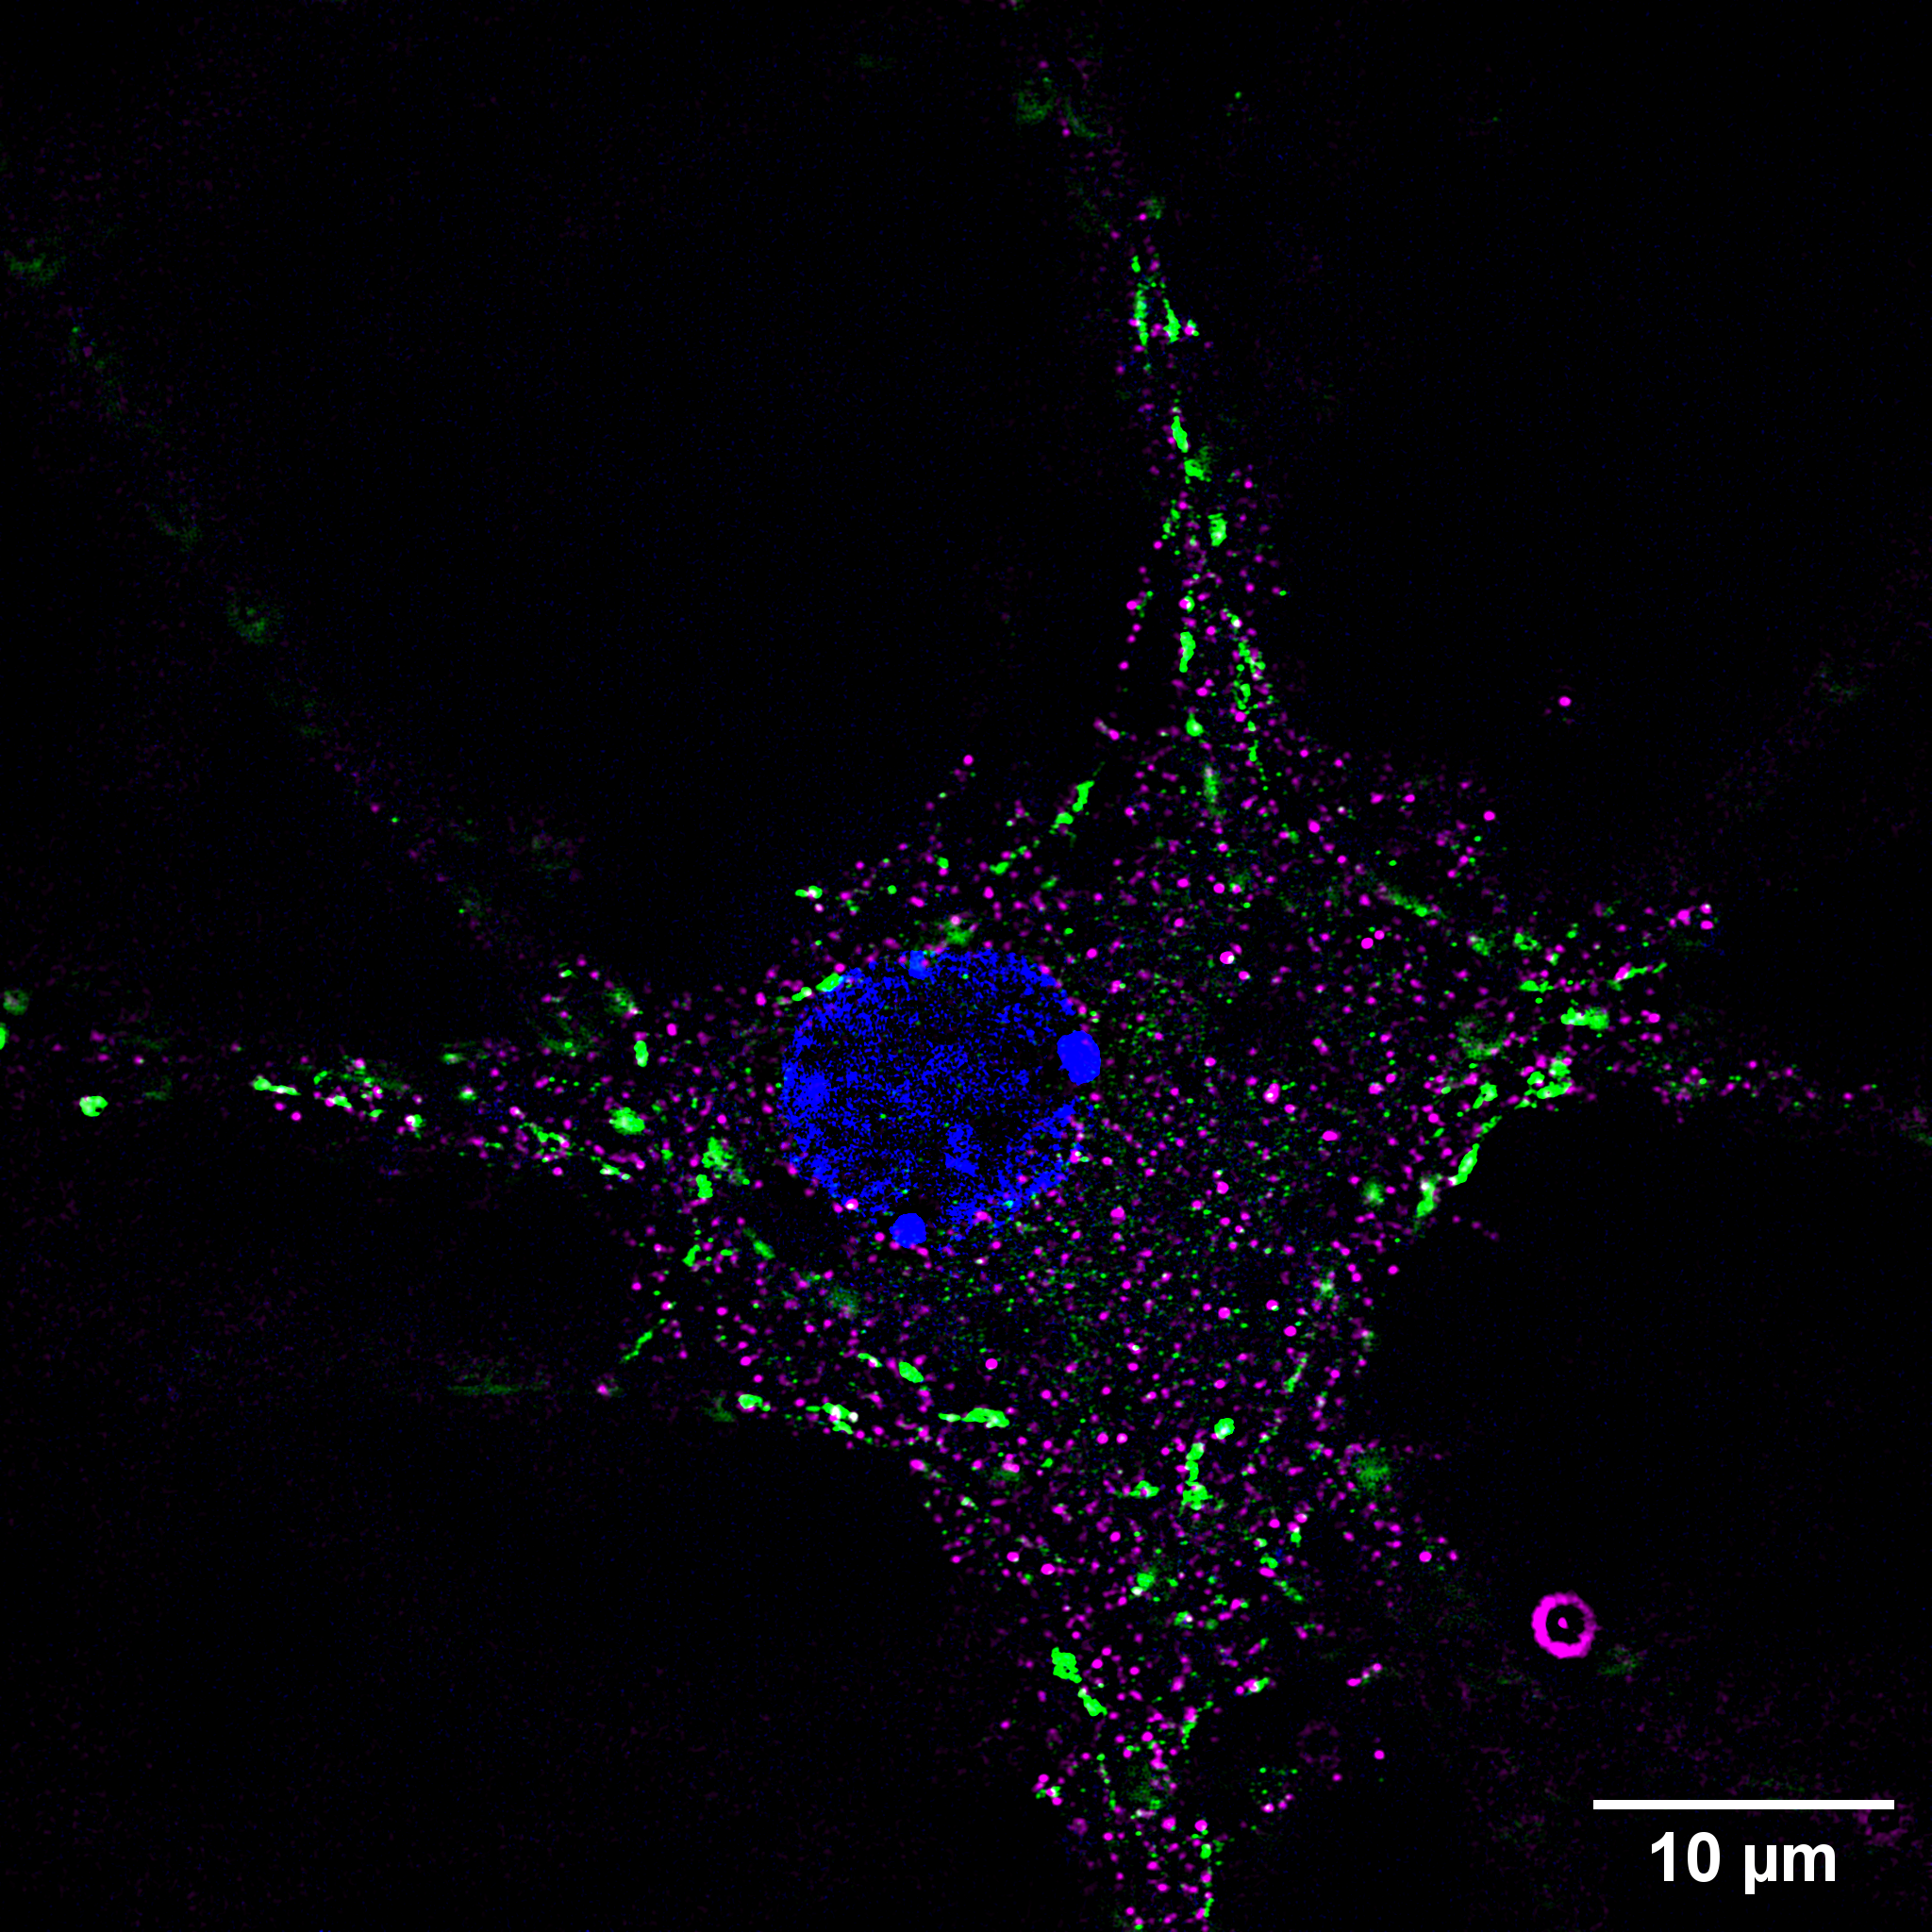
\includegraphics[width=0.8\textwidth]{abbildungen/SIMNervEuA.png} % Lädt das Bild, skaliert es auf 80% der Textbreite
	\caption{Structured-Illumination-Microscopie-(SIM)-Aufnahme einer Nervenzelle. Die fluoreszierenden Strukturen zeigen Caspr2 (magenta), VGat (grün) und einen Zellkern (blau) \parencite{eigenAu7.3}} % Die Bildunterschrift
	\label{fig:SIMnerv} % Ein Label für Querverweise (z.B. "siehe Abbildung \ref{fig:beispielbild}")
\end{figure}
% ── Abbildung 2 (Mann-Whitney U-Test Screenshot) ausgelassen ─
% Abb. 2: Mann-Whitney U-Test von SIM in OriginPro 2019
% 
%%	\centering % Zentriert das Bild horizontal
%	\label{fig:mwutma} % Ein Label für Querverweise (z.B. "siehe Abbildung \ref{fig:beispielbild}")
%\end{figure}
\clearpage
\section{Kolokalisation von Caspr2 und Contactin-2 nach der
	Behandlung mit verschiedenen Antikörpern}

Zur Untersuchung des Effekts der Anti-Caspr2-aAK auf die Interaktion
zwischen Caspr2 und Contactin-2 wurden Neuronenkulturen von Mäusen
entweder mit AK gegen die Discoidin- oder die Laminin-Domäne von Caspr2
behandelt. Mittels SIM wurden hochauflösende Aufnahmen der Synapsen gemacht. Die Kolokalisationsflächen wurden mittels IMARIS analysiert.

Bei der Überprüfung der Werte mittels Shapiro-Wilk-Tests lag keine
Normalverteilung vor, daher erfolgte erneut ein Vergleich zwischen den
Gruppen mittels Mann-Whitney U-Test.

Die Kolokalisationsflächen in Abbildung \ref{fig:aAKstat} weisen in beiden Gruppen ähnliche Wertebereiche auf. Bei den Antikörpern, die an die Discoidin-Domäne
binden, liegt der Median bei ca.\ $1{,}8\,\mu\text{m}^2$, die mittleren
50\,\% der Werte liegen in etwa zwischen
$1{,}4$--$2{,}5\,\mu\text{m}^2$ und es liegt ein Wert außerhalb des
Hauptbereichs bei rund $5\,\mu\text{m}^2$.

Die Laminin-Werte sind zahlreicher und deutlich stärker gestreut. %...............(diskussion dann später)
Der Median der Laminin-Werte liegt bei
$1{,}6\,\mu\text{m}^2$. Die mittleren 50\,\% der Werte liegen im
Vergleich zu den Discoidin-Werten in einem geringeren Bereich. Der
Bereich reicht von etwa $1{,}2$--$2{,}2\,\mu\text{m}^2$.

Der Mann-Whitney U-Test zeigt keinen signifikanten
Unterschied zwischen den Werten von AK, die an die Discoidin- oder
Laminin-Domäne binden ($p = 0{,}386$, n.\,s.).

Der Mann-Whitney U-Test liefert keinen statistischen Nachweis für einen unterschiedlichen Effekt der AK-Gruppen. Eine mögliche Tendenz ist aufgrund vermehrter Einzelwerte und einer größeren Streuung der Werte in den Proben der Laminin-AK zu vermuten. Dennoch lässt sich hier keine eindeutige Aussage treffen.

% ── Abbildung 3 (Boxplot Discoidin/Laminin) ausgelassen ──────
% Abb. 3: Einfluss von Anti-Caspr2-aAK gegen die Discoidin-
%         bzw. Laminin-Domäne von Caspr2 auf die Kolokalisation
%         mit Contactin-2
% ─────────────────────────────────────────────────────────────
\begin{figure}[h] % [h] versucht, das Bild hier zu platzieren (hier), [t] für oben, [b] für unten
	\centering % Zentriert das Bild horizontal
	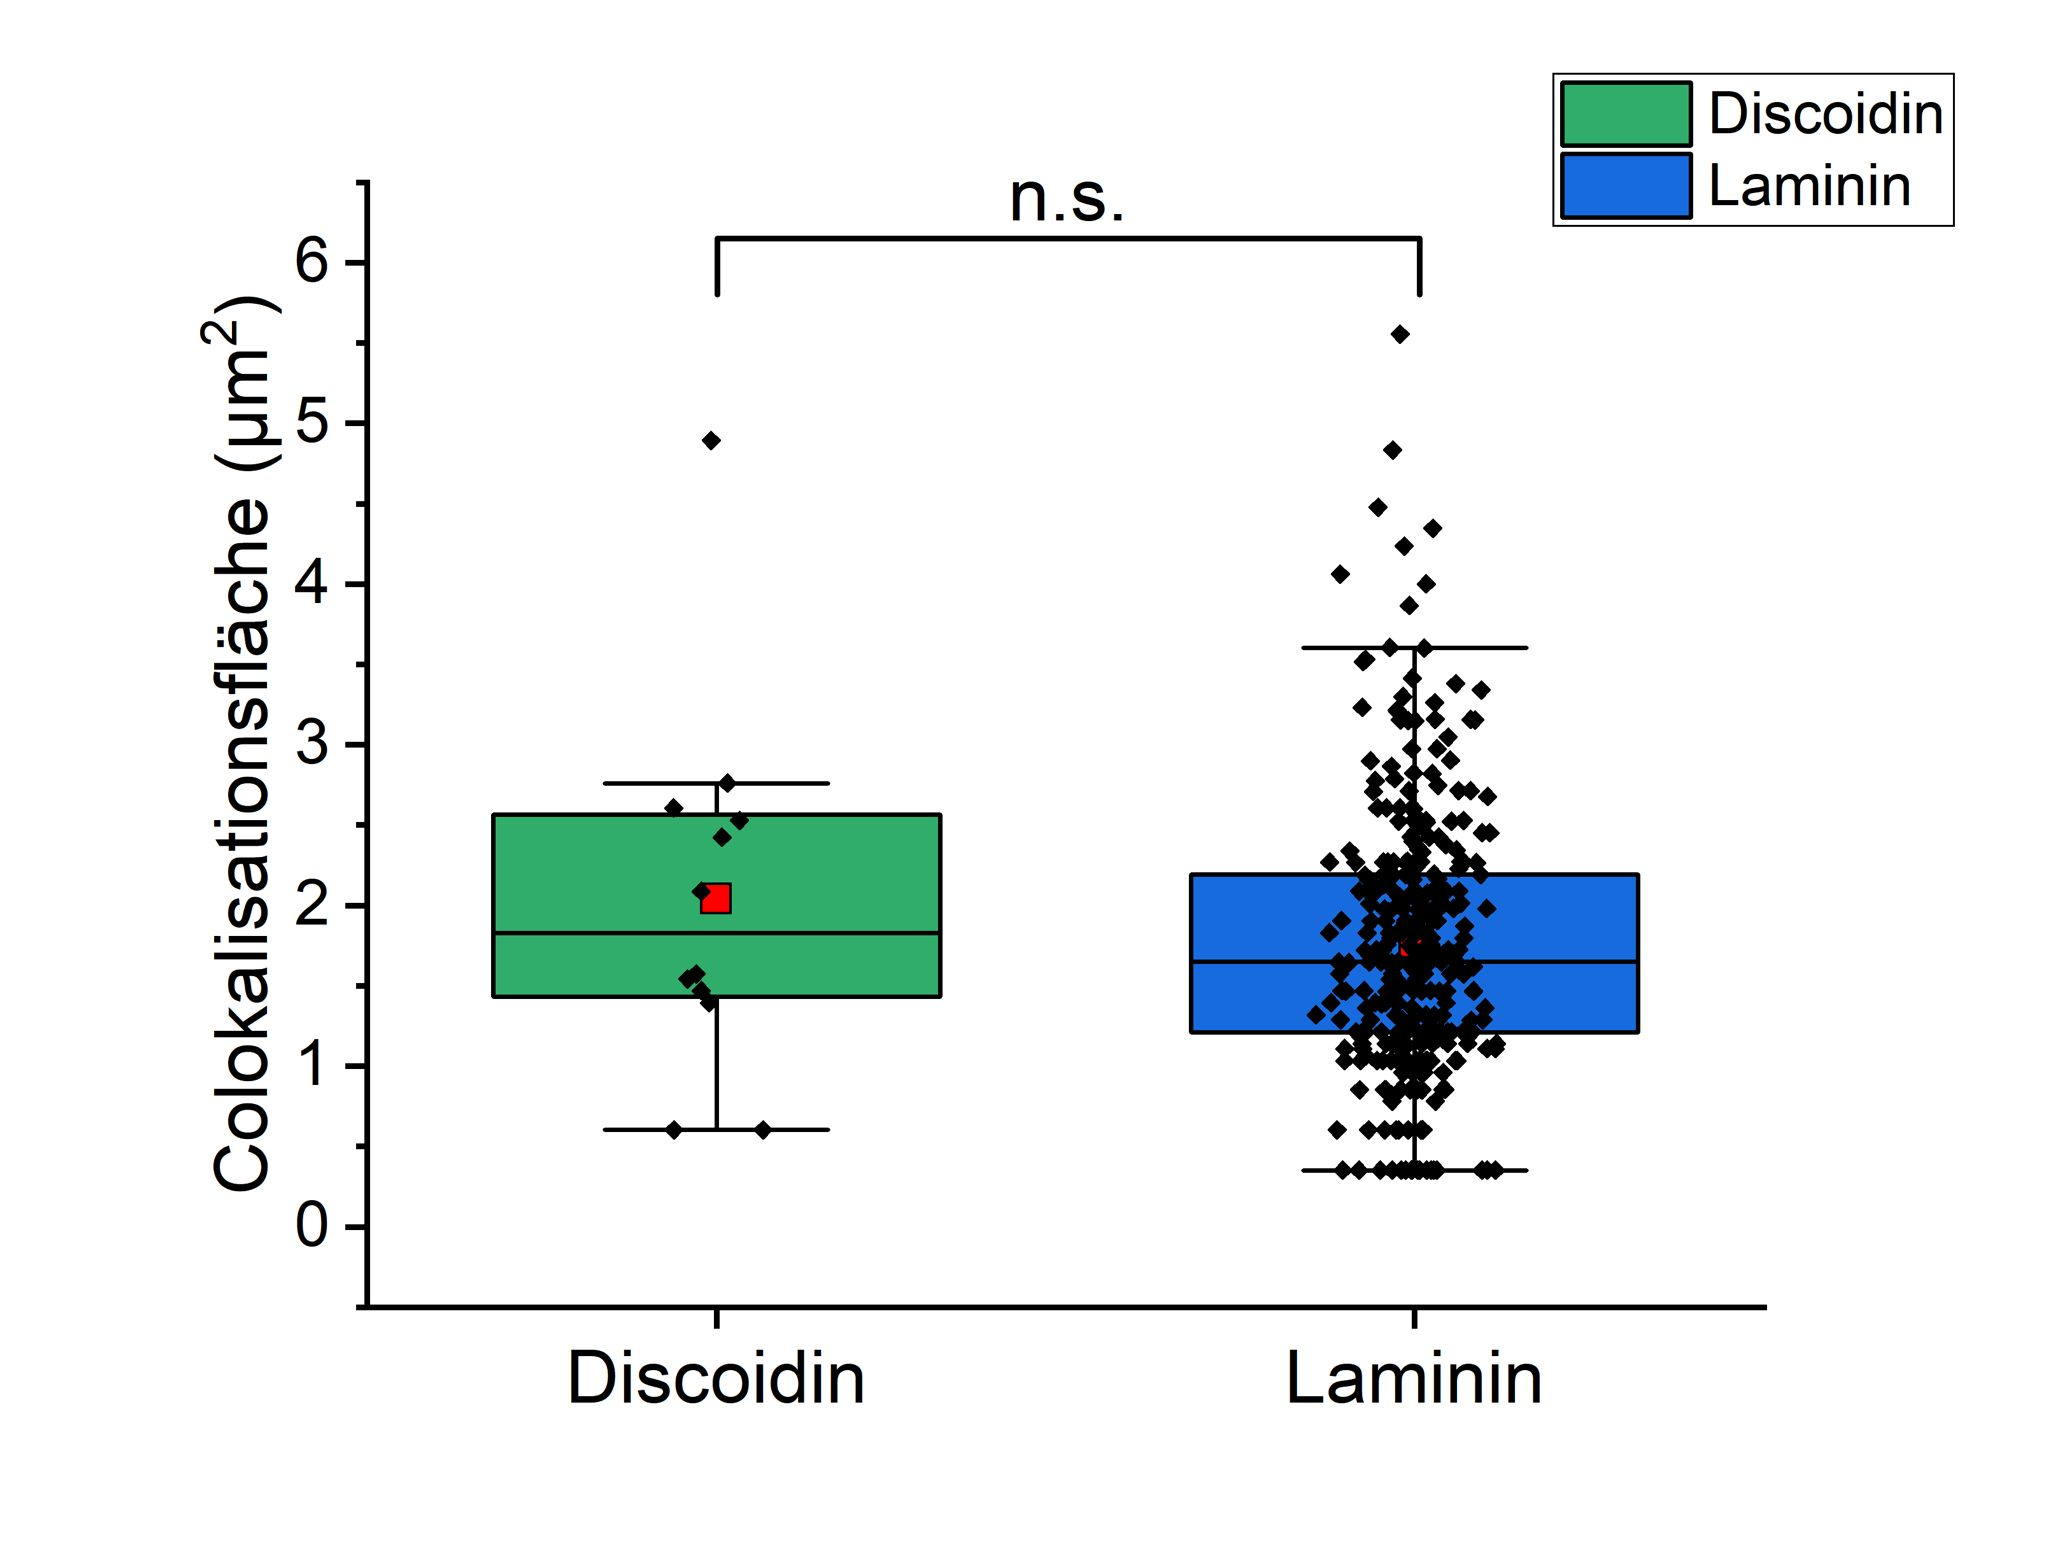
\includegraphics[width=0.91\textwidth]{abbildungen/aAKstatKCVV.jpg} % Lädt das Bild, skaliert es auf 80% der Textbreite
	\caption{Einfluss von Anti-Caspr2-aAK gegen die Discoidin- bzw. Laminin-Domäne
		von Caspr2 auf die Kolokalisation mit Contactin-2 \parencite{eigenAu7.4}} % Die Bildunterschrift
	\label{fig:aAKstat} % Ein Label für Querverweise (z.B. "siehe Abbildung \ref{fig:beispielbild}")
\end{figure}

% ── Abbildung 4 (Mann-Whitney U-Test Screenshot) ausgelassen ─
% Abb. 4: Mann-Whitney U-Test in OriginPro 2019
% ─────────────────────────────────────────────────────────────
%\begin{figure}[h] % [h] versucht, das Bild hier zu platzieren (hier), [t] für oben, [b] für unten
%	\centering % Zentriert das Bild horizontal
%	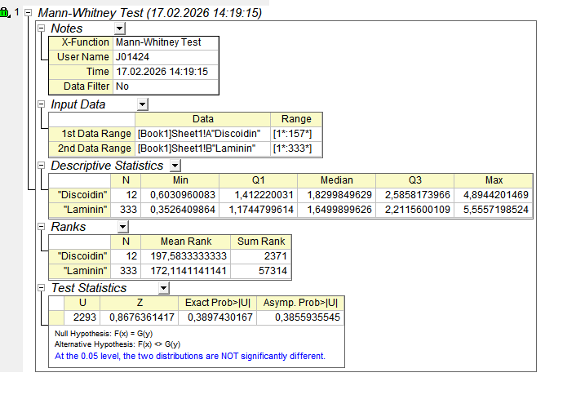
\includegraphics[width=0.91\textwidth]{abbildungen/mwutestaAK.png} % Lädt das Bild, skaliert es auf 80% der Textbreite
%	\caption{Mann-Whitney U-Test von SIM in OriginPro 2019 auf der Einfluss von Anti-Caspr2-aAK \parencite{eigenAu7.4}} % Die Bildunterschrift
%	\label{fig:mwutaAK} % Ein Label für Querverweise (z.B. "siehe Abbildung \ref{fig:beispielbild}")
%\end{figure}
 
\clearpage
%Um die Lokalisation zu bestimmen, wurde jeweils Caspr2 und vesikuläre
%GABA-Transporter (VGat) oder vesikuläre Glutamattransporter (VGlut)
%angefärbt. VGat dient dabei als Marker für inhibitorische Synapsen und
%VGlut als Marker für exzitatorische Synapsen. Mittels Bestimmung der
%Kolokalisationsfläche der fluoreszierenden Farbstoffe lässt sich
%ermitteln, an welcher Synapsenart Caspr2 vorwiegend vorliegt.
%
%In Abb.~1 ist jeweils die Größe einzelner sowie die Anzahl an
%Kolokalisationsflächen ($\mu\text{m}^2$) von Caspr2 mit den
%Synapsenmarkern VGat (schwarz) und VGlut (rot) bei den
%Mikroskopieverfahren Structured Illumination Microscopy (SIM) und Wide
%Field (WF) dargestellt.
%
%Die durchschnittliche Kolokalisationsfläche von VGat ist bei der
%SIM-Mikroskopie ähnlich groß wie die VGlut-Kolokalisationsfläche und
%liegt bei ca.\ $1\,\mu\text{m}^2$. Die Kolokalisationsflächen von Caspr2
%und VGat sind teils größer und es wurden deutlich mehr
%Kolokalisationsflächen gefunden. Bei der VGlut-Analyse findet sich
%lediglich ein Wert.
%% Anmerkung: Färbung hat nicht sonderlich gut funktioniert – 
%%            Fehlerbetrachtung einfügen.
%
%Bei der WF-Mikroskopie lässt sich eine starke Streuung der Größe der
%Kolokalisationsflächen von VGat und Caspr2 finden. Des Weiteren liegen
%teilweise sehr große Kolokalisationsflächen vor. Der Median der
%VGat-Kolokalisation ist minimal höher als der der VGlut-Kolokalisation,
%beide liegen im Bereich von ca.\
%$1{,}5$--$2\,\mu\text{m}^2$. Die Größen der
%VGlut-Kolokalisationsflächen liegen im moderaten Bereich und weisen eine
%geringere Streuung als bei VGat auf. Sowohl bei der WF- als auch bei der
%SIM-Mikroskopie ist die Anzahl an Kolokalisationsflächen bei VGat
%erkennbar höher.
%
%Die erhöhte Anzahl an VGat-Kolokalisation ist im Kontext zu sehen. Die
%Synapsendichte an inhibitorischen Synapsen könnte in den Aufnahmen größer
%gewesen sein als die der exzitatorischen Synapsen. Die Mediane der
%Flächengrößen sind annähernd gleich.
\include{kapitel/Diskussion.tex}
\include{kapitel/Fazit_und_Ausblick.tex}
\include{kapitel/Anhang.tex}

    
    
        
        
        













\chapter{Literaturverzeichnis}
%\nocite{*}
\printbibliography[heading=none , notkeyword={bild}]
%% Manuelle Formatierung mit hängendem Einzug (sieht professionell aus)
%\setlength{\parindent}{0pt} % Kein Einzug der ersten Zeile
%\setlength{\parskip}{6pt}   % Abstand zwischen den Einträgen
%Reichert, Heinrich (2000): \textit{Neurobiologie.} 2. Aufl. Stuttgart / New York: Thieme.
%
%Sell, Josephine (2023): \textit{Zelluläre Pathomechanismen von humanen Autoantikörpern gegen LGI1 und GABAB-Rezeptoren bei autoimmunen Enzephalitiden.} 1. Aufl. Jena: Friederich-Schiller-Universität Jena, Universitätsklinikum Jena.
%
%Joppien, Saskia / Maier, Sarah Lena / Wendling, Danielle Sabina (2011): \textit{BASICS Experimentelle Doktorarbeit.} 1. Aufl. München: Urban \& Fischer Verlag.
%
%
%Mulisch, Maria / Welsch, Ulrich (Hrsg.), (2010): \textit{Romeis Mikroskopische Technik.} 18. Aufl. Heidelberg: Spektrum Akademischer Verlag.
%
%
%
% van Sonderen, Agnes / Petit-Pedrol, Mar / Dalmau, Josep / Titulaer, Maarten J. (2016): \textit{The value of LGI1, Caspr2 and voltage-gated potassium channel antibodies in encephalitis.} In: Nature Reviews Neurology, Advance Online Publication, S. 1--12.
%
%
%Lehrbuch (Markl (1997): S. )
%Markl, Jürgen (Original englisch von: Campbell, Neil A.) (1997): Biologie. ?. Spektrum Akademischer Verlag Heidelberg. Berlin
%
%(Westphalen/DocCheck Flexikon (03.01.2026))
%Graf von Westphalen, Georg et al. In: DocCheck Flexikon - Nervensystem. \url{https://flexikon.doccheck.com/de/Nervensystem}
%[Abrufdatum: 03.01.2026].
%
%(Freedman/MSD Manuals (03.01.2026))
%Freedman, Mark (2025): Rückenmark. \url{https://www.msdmanuals.com/de/heim/störungen-der-hirn-rückenmarks-und-nervenfunktion/biologie-des-nervensystems/rückenmark}
%[Abrufdatum 03.01.2026].
%
%(Högelmann/DocCheck Flexikon (03.01.2026))
%Högelmann, Astrid et al. In: DocCheck Flexikon - Hippocampus. \url{https://flexikon.doccheck.com/de/Hippocampus}
%[Abrufdatum 03.01.2026].
%
%(Cell Signaling Technololgy (10.01.2026))
%Cell Signal Technology. Caspr2 Antikörper \#3731. Hintergrung. \url{https://www.cellsignal.com/products/primary-antibodies/caspr2-antibody/3731}
%[Abrufdatum 10.01.2026].
%
%(Saint-Martin/PubMed (10.01.2026))
%Saint-Martin, Margaux et al. (2019): Impact of anti-CASPR2 autoantibodies from patients with autoimmune encephalitis on CASPR2/TAG-1 interaction and Kv1 expression. \url{https://pubmed.ncbi.nlm.nih.gov/31176559/}
%[Abrufdatum 10.01.2026].
%
%
%(Freedman2/MSD Manuals (03.01.2026))
%Freedman, Mark (2025): Nerven. \url{https://www.msdmanuals.com/de/heim/störungen-der-hirn-rückenmarks-und-nervenfunktion/biologie-des-nervensystems/nerven}
%[Abrufdatum 03.01.2026].
%
%(Hircin/DocCheck Flexikon (10.01.2026))
%Hircin, Emrah et al. In: DocCheck Flexikon - Aktionspotential. \url{https://flexikon.doccheck.com/de/Aktionspotential}
%[Abrufdatum 10.01.2026].
%
%(Antwerpes/DockCheck Flexikon (10.01.2026))
%Antwerpes, Frank et al. In: DocCheck Flexikon - Membranpotential. \url{https://flexikon.doccheck.com/de/Membranpotential}
%[Abrufdatum 10.01.2026].
%
%(Haklai-Topper/PubMed Central (12.01.2026))
%Haklai-Topper, Liat (2010): The Neurexin superfamily of Caenorhabditis elegans. \url{https://pmc.ncbi.nlm.nih.gov/articles/PMC12414531/}
%[Abrufdatum 12.01.2026].
%
%Macian et al. (2004):
%Macian, Fernando / García-Cozar, Francisco / Im, Seon-Hee / et al. (2004): T cell anergy. In: Investigación clínica, 45.1, S. 1–2. \url{https://pubmed.ncbi.nlm.nih.gov/15023415/}
%[Abrufdatum 14.01.2026].
%
%Wikipedia2026:
%Autoimmunerkrankung (14. Januar 2026). In: Wikipedia – Die freie Enzyklopädie. \url{https://de.wikipedia.org/wiki/Autoimmunerkrankung}
%[Abrufdatum 14.01.2026].
%
%DocCheckLymphozyt:
%Lymphozyt (14. Januar 2026). In: DocCheck Flexikon. \url{https://flexikon.doccheck.com/de/Lymphozyt}
%[Abrufdatum 14.01.2026].
%
%MSD Gesundheit (12.01.2026):
%MSD Gesundheit. Definition und häufigste Formen. \url{https://www.msd-gesundheit.ch/de/immunologie/Definition-und-h%C3%A4ufigste-Formen}
%[Abrufdatum 14.01.2026].
%
%MSD Manuals Autoimmunerkrankungen(12.01.2026):
%MSD Manuals. Autoimmunerkrankungen. \url{https://www.msdmanuals.com/de/heim/immunst%C3%B6rungen/allergische-reaktionen-und-andere-hypersensitivit%C3%A4tsst%C3%B6rungen/autoimmunerkrankungen}
%[Abrufdatum 14.01.2026].
%
%MSD Manuals Immunsystem(12.01.2026):
%MSD Manuals. Überblick über das Immunsystem. \url{https://www.msdmanuals.com/de/profi/immunologie-allergien/biologie-des-immunsystems/%C3%BCberblick-%C3%BCber-das-immunsystem}
%[Abrufdatum 14.01.2026].
%
%UniHeidelbergImmunologie2026:
%Universitätsklinikum Heidelberg. Übersicht Sektion Molekulare Immunologie. \url{https://www.klinikum.uni-heidelberg.de/immunologie/forschung/sektion-molekulare-immunologie/uebersicht}
%[Abrufdatum 14.01.2026].
%
%
%Klein/MSD Manual (10.01.2026):
%MSD Manual. Gehirnentzündung (Enzephalitis).
%\url{https://www.msdmanuals.com/de/heim/störungen-der-hirn-rückenmarks-und-nervenf
%unktion/infektionen-des-gehirns/gehirnentzündung-enzephalitis#Arten-der-Enzephalit
%is_v26247328_de} [Abrufdatum: 10.01.2026]
%
%Fernandez/MSD Manual (10.01.2026):
%MSD Manual. Autoimmunerkrankungen.
%\url{https://www.msdmanuals.com/de/heim/immunstörungen/allergische-reaktionen-undandere-hypersensitivitätsstörungen/autoimmunerkrankungen?_gl=1*1gp4ebm*_up*
%MQ..*_ga*MTE2NzI1MzQ4Ni4xNzY3OTQ1NDYz*_ga_CJ792HFYYC*czE3Njc5NDU
%0NjMkbzEkZzAkdDE3Njc5NDU0NjMkajYwJGwwJGgw} [Abrufdatum: 10.01.2026]
%
%Heine (2022):
%Heine, Josephine / Duchow, Ankelien / Rust, Rebekka / Paul, Friedemann / Prüß,
%Harald / Finke, Carsten (2022): Autoimmunenzephalitis - ein Update.
%\url{https://pmc.ncbi.nlm.nih.gov/articles/PMC9748390/} [Abrufdatum: 15.12.2025]
%
%Graus (2016):
%Graus, Francesc et al. (2016): A clinical approach to diagnosis of autoimmune
%encephalitis.
%\url{https://www.thelancet.com/action/showPdf?pii=S1474-4422%2815%2900401-9}
%[Abrufdatum: 10.01.2026]
%
%Universitätsklinikum Heidelberg (10.01.2026):
%Universitätsklinikum Heidelberg. Autoimmunenzephalitis.
%\url{https://www.klinikum.uni-heidelberg.de/erkrankungen/autoimmunenzephalitis-202062
%#:~:text=Die%20Therapie%20erfolgt%20stufenweise.,das%20Immunsystem%20län
%gerfristig%20herabregulieren%20(sog.} [Abrufdatum: 10.01.2026]
%
%Generate Net (10.01.2026):
%Generate Net. Wie werden verschiedene Krankheitsbilder diagnostiziert?.
%\url{https://generate-net.de/wie-werden-die-verschiedenen-krankheitsbilder-diagnostiziert
%.html} [Abrufdatum: 10.01.2026]
%
%Lancaster (2015):
%Lancaster, Eric (2015): The Diagnosis and Treatment of Autoimmune Encephalitis.
%\url{https://www.thejcn.com/DOIx.php?id=10.3988/jcn.2016.12.1.1} [Abrufdatum:
%10.01.2026]
%
%van Sondern (2016):
%van Sondern, Agnes / Arino, Helena et al. (2016): The clinical spectrum of Caspr2
%antibody-associated disease. \url{https://pmc.ncbi.nlm.nih.gov/articles/PMC4970662/}
%[Abrufdatum: 10.01.2026]

\chapter{Bildquellenverzeichnis}
\begin{refcontext}[sorting=bylabel]
	\printbibliography[heading=none, env=bildliste, keyword=bild]
\end{refcontext}


%Abbildung 2.1: medi-karriere.de: Grafik eines Neurons. Oktober 2024. Zit. nach Medi-Karriere. \url{https://www.medi-karriere.de/wp-content/uploads/2024/10/Grafik-Neuron-2-e1730282985666.jpg} [Abrufdatum 14.01.2026].
%
%Abbildung 2.2: sofatutor.net: Phagozytose. 2024. Zit. nach sofatutor. \url{https://images.cdn.sofatutor.net/content_images/images/22218/original/Phagozytose.svg?1744379262} [Abrufdatum 14.01.2026].
%
%Abbildung 3.1: generate-net.de: Klinischer Verdacht auf immunvermittelte Encephalitis. 2024. Zit. nach Generate-Net. \url{https://generate-net.de/files/grafiken/Klinischer%20Verdacht%20auf%20immunvermittelte%20Encephalitis.png} [Abrufdatum 14.01.2026].

\end{document}
